% !TeX spellcheck = en_GB
%%%%%%%%%%%%%%%%%%%%%%%%%%%%%%%%%%%%%%%%%%
%                                        %
%    Engineer thesis LaTeX template      % 
%                                        %
%%%%%%%%%%%%%%%%%%%%%%%%%%%%%%%%%%%%%%%%%%



\documentclass[a4paper,twoside,12pt]{book}
\usepackage[utf8]{inputenc}                                      
\usepackage[T1]{fontenc}  
\usepackage{amsmath,amsfonts,amssymb,amsthm}
% \usepackage[polish,british]{babel} 
\usepackage{indentfirst}
\usepackage{lmodern}
\usepackage{graphicx}
\usepackage{subcaption}
\captionsetup{compatibility=false}
\usepackage{float}
\usepackage{hyperref}
\usepackage{booktabs}
\usepackage{tikz}
\usepackage{pgfplots}
\usepackage{mathtools}
\usepackage{geometry}
\usepackage[page]{appendix} 
\usepackage[backend=bibtex]{biblatex}
\addbibresource{thebibliography.bib}

\usepackage{setspace}
\onehalfspacing


\frenchspacing

\usepackage{listings}
\lstset{
	language={},
	basicstyle=\ttfamily,
	keywordstyle=\lst@ifdisplaystyle\color{blue}\fi,
	commentstyle=\color{gray}
}

% Helps when line is to wide and can't be broken properly
\setlength{\emergencystretch}{10pt}
%%%%%%%%%

 

%%%%%%%%%%%% FANCY HEADERS %%%%%%%%%%%%%%%

\usepackage{fancyhdr}
\pagestyle{fancy}
\fancyhf{}
\fancyhead[LO]{\nouppercase{\it\rightmark}}
\fancyhead[RE]{\nouppercase{\it\leftmark}}
\fancyhead[LE,RO]{\it\thepage}
\setlength{\headheight}{15pt}% at least 14.49998pt


\fancypagestyle{onlyPageNumbers}{%
   \fancyhf{} 
   \fancyhead[LE,RO]{\it\thepage}
}

\fancypagestyle{PageNumbersChapterTitles}{%
   \fancyhf{} 
   \fancyhead[LO]{\nouppercase{\it\rightmark}}
   \fancyhead[RE]{\nouppercase{\it\leftmark}}
   \fancyhead[LE,RO]{\it\thepage}
}


%%%%%%%%%%%%%%%%%%%%%%%%%%%
% listings 
\usepackage{listings}
\lstset{%
language=C++,%
% commentstyle=\textit,%
% identifierstyle=\textsf,%
% keywordstyle=\sffamily\bfseries, %\texttt, %
commentstyle=\itshape\color{purple!40!black},%
identifierstyle=\color{blue},%
keywordstyle=\bfseries\color{green!40!black},%
stringstyle=\color{orange},
%captionpos=b,%
tabsize=3,%
frame=lines,%
numbers=left,%
numberstyle=\tiny,%
numbersep=5pt,%
breaklines=true,%
morekeywords={uint8_t, uint16_t, uint32_t, int8_t, int16_t, int32_t, float32_t, __attribute__, section, aligned},%
escapeinside={@*}{*@},%
texcl=true, % wylacza tryb verbatim w komentarzach jednolinijkowych
}
%%%%%%%%%%%%%%%%%%%%%%%%%%%%%%%%%%%%

% % %%%% TODO LIST GENERATOR %%%%%%%%%

% % \usepackage{color}
% % \definecolor{brickred}      {cmyk}{0   , 0.89, 0.94, 0.28}

% % \makeatletter \newcommand \kslistofremarks{\section*{Remarks} \@starttoc{rks}}
% %   \newcommand\l@uwagas[2]
% %     {\par\noindent \textbf{#2:} %\parbox{10cm}
% % {#1}\par} \makeatother


% % \newcommand{\remark}[1]{%
% % {%\marginpar{\textdbend}
% % {\color{brickred}{[#1]}}}%
% % \addcontentsline{rks}{uwagas}{\protect{#1}}%
% % }

% % %%%%%%%%%%%%%% END OF TODO LIST GENERATOR %%%%%%%%%%% 

% % % some issues...

\newcounter{PagesWithoutNumbers}

\newcommand{\hcancel}[1]{%
    \tikz[baseline=(tocancel.base)]{
        \node[inner sep=0pt,outer sep=0pt] (tocancel) {#1};
        \draw[red] (tocancel.south west) -- (tocancel.north east);
    }%
}%

\newcommand{\MonthName}{%
  \ifcase\the\month
  \or January% 1
  \or February% 2
  \or March% 3
  \or April% 4
  \or May% 5
  \or June% 6
  \or July% 7
  \or August% 8
  \or September% 9
  \or October% 10
  \or November% 11
  \or December% 12
  \fi}


%%%%%%%%%%%%%%%%%%%%%%%%%%%%%%%%%%%%%%%%%%%%%%
% Helvetica font macros for the title page:
\newcommand{\headerfont}{\fontfamily{phv}\fontsize{18}{18}\bfseries\scshape\selectfont}
\newcommand{\titlefont}{\fontfamily{phv}\fontsize{18}{18}\selectfont}
\newcommand{\otherfont}{\fontfamily{phv}\fontsize{14}{14}\selectfont}

%%%%%%%%%%%%%%%%%%%%%%%%%%%%%%%%%%%%%%%%%%%%%%
%%%%%%%%%%%%%%%%%%%%%%%%%%%%%%%%%%%%%%%%%%%%%%
%%%%%%%%%%%%%%%%%%%%%%%%%%%%%%%%%%%%%%%%%%%%%%
%%%%%%%%%%%%%%%%%%%%%%%%%%%%%%%%%%%%%%%%%%%%%%
%%%%%%%%%%%%%%%%%%%%%%%%%%%%%%%%%%%%%%%%%%%%%%
%%%%%%%%%%%%%%%%%%%%%%%%%%%%%%%%%%%%%%%%%%%%%%
%%%%%%%%%%%%%%%%%%%%%%%%%%%%%%%%%%%%%%%%%%%%%%


\newcommand{\Author}{Michał Mieszczak}
\newcommand{\Supervisor}{dr inż. Jerzy Fiołka}
\newcommand{\Consultant}{Name Surname, PhD}
\newcommand{\Title}{Realization of digital audio effects on high-performance MCU platform.}
\newcommand{\Polsl}{Silesian University of Technology}
\newcommand{\Faculty}{Faculty of Automatic Control, Electronics and Computer Science}


% Deals with some compatibility warning
\pgfplotsset{compat=1.16}

\begin{document} 
	
%%%%%%%%%%%%%%%%%%  Title page %%%%%%%%%%%%%%%%%%% 
\pagestyle{empty}
{
	\newgeometry{top=2.5cm,%
	             bottom=2.5cm,%
	             left=3cm,
	             right=2.5cm}
	\sffamily
	\rule{0cm}{0cm}
	
	\begin{center}
	
\includegraphics[width=29mm]{polsl}
	\end{center} 
	\vspace{1cm}
	\begin{center}
	\headerfont \Polsl
	\end{center}
	\begin{center}
	\headerfont \Faculty
	\end{center}
	\vfill
	\begin{center}
	\titlefont Engineer  thesis
	\end{center}
	\vfill
	
	\begin{center}
	\otherfont \Title\par
	\end{center}
	
	\vfill
	
	\vfill
	 
	\noindent\vbox
	{
		\hbox{\otherfont Author: \Author}
		\vspace{12pt}
		\hbox{\otherfont Supervisor: \Supervisor}
		% \vspace{12pt}
		% \hbox{\otherfont consultant: \Consultant}
	}
	\vfill 
 
   \begin{center}
   \otherfont Gliwice,  \MonthName\ \the\year
   \end{center}	
   \restoregeometry
}
  

\cleardoublepage
 
\rmfamily
\normalfont

%%%%%%%%%%%%%%%%%% Table of contents %%%%%%%%%%%%%%%%%%%%%%
\pagenumbering{Roman}
\pagestyle{onlyPageNumbers}
\tableofcontents

%%%%%%%%%%%%%%%%%%%%%%%%%%%%%%%%%%%%%%%%%%%%%%%%%%%%%
\setcounter{PagesWithoutNumbers}{\value{page}}
\mainmatter
\pagestyle{PageNumbersChapterTitles}



\chapter{Introduction}
The rapid development of technology lead to the moment, when anybody can afford a development board 
and learn how to program microcontrollers without even leaving house.
Hobbysts all around the world create products in wide range of applications, that can easily compete
with their professional counterparts in both price and quality.

One example of such a field is market of sound related equipment.
More and more small companies are growing out of nowhere,
providing butique studio recording and processing equipment with great customer service and support.




\chapter{Goals and tasks of the project}
The main goal of the project is to develop a platform based around modern,
high-performance microcontroller.
The device should process stereo audio signal to achieve a selection of different effects
while delivering decent sound quality.
Following tasks are required to finish the project:

\begin{enumerate}
    \item Choice of components
    \begin{itemize}
        \item microcontroller
        \item operational amplifiers
        \item additional devices
    \end{itemize}

    \item List of features
    \begin{itemize}
        \item list of audio effects
        \item user interface
    \end{itemize}

    \item Creating the physical layer of device
    \begin{itemize}
        \item block diagram
        \item schematic
        \item PCB
        \item assembly 
    \end{itemize}

    \item Developing software
    \begin{itemize}
        \item choosing programming language
        \item choosing IDE, text editor, toolchain and frameworks
        \item writing and testing the program (user interface, effects)
    \end{itemize}
\end{enumerate}




\chapter{Topic analysis}
This chapter is devoted to main concerns related to the project,
that need to be considered at the beginning.
These will determine all important features and parameters of the device.

\section{Data acquisition}
The nature of audio signal is analog. This means,
that it should be conditioned in a proper way before it can be processed by digital circuitry.
It is done by ADC and coresponding preamplifier.

Signal must be reduced from continuous-time to discrete-time.
This process is called sampling and requires reading value of the signal in equal intervals of time.
Range of audible frequencies is considered to be 20Hz to 20kHz
and we need the whole range to acheive reasonable quality.
According to the concept of Nyquist frequency, the sampling frequency should be at least
twice as high as maximum frequency present in the signal.
In case of audio signal, it must be at leasu 40kHz.
There are some typical sampling frequencies preffered for audio signals such as: 44,1kHz, 48kHz,
96kHz, 192kHz and it would be a good idea to use one of them.

Furthermore ADC quantizes the value of the signal.
This means, that signal can take one of finite number of values.
The count of possible values is equal to \(2^n\), where n is the bit depth of the converter.

As stereo signal consists of two separate channels,
there sould be two identical sets of preaplifiers and converters.

\section{Output generation}
Processed digital signal must be converted back to analog.
This is done using DAC and corresponding amplifier.
DAC converts digital value into specific analog voltage,
outputs it and holds the value until succesive sample is to be outputted.

\section{Processing audio}
Digital signals are usually processed in blocks.
This approach allows to use FFT, which is necessary for some effects.
Furthermore it can reduce time needed to process each sample.
One drawback of this method is latency introduced.
The whole block of samples needs to be collected before it can be processed.
In case of blocks consisting of 512 samples,
there is 1024 samples delay between collecting and outputting specific sample.
In combination with 48kHz sampling frequency this results in 21.3 ms latency.
Outputting, processing and collecting subsequent blocks off data
must be performed simultaneously.

Data collected from converters is represented as unsigned integer values.
For 16 bit converter we get values between 0 and 16536 (\(2^16\)).
Such format is not suitable for processing.
To deal with it, samples should be first converted into fixed or floating-point values.
Fixed-point data type can represent fractional values in range from -1 to 1.
Main disadvantage of fixed-point approach is easy overflow.
These problem can be eliminated by using floating-point numbers instead.
Floating-point introduces exponent bits alongside with mantissa (fraction bits).
\cite{ST:DSP}

\begin{figure}[H]
    \centering
    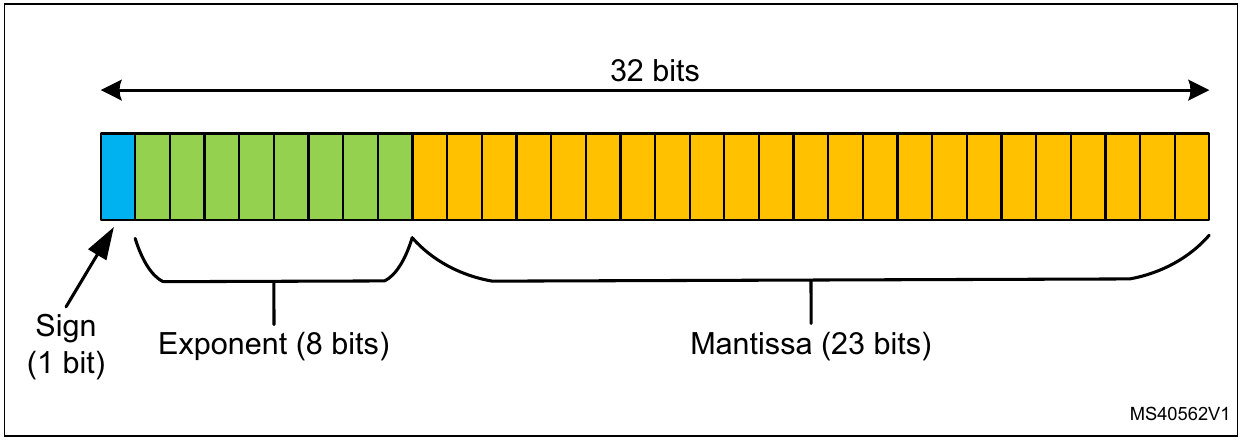
\includegraphics[width=\textwidth]{images/float}
    \caption{32-bit floating-point representation.}
    \label{fig:Float}
\end{figure}

\section{Effects}
This section is dedicated to audio effects implemented in the devices
as well as their features and parameters.
It is important to fully understand nature of specific effect
in order to implement it's entire functionality in a proper way.
\cite{Zolzer1}
\cite{Zolzer2}
\cite{Smith}

\subsection{Delay}
Delay is the most basic time based effects.
It creates echo of original signal,
which is delayed by specified amount of time.
This delayed signal is then mixed with original.
Delayed signal can also be attenuated and then fed back into a delay block
in order to achieve endless, fading reflections.

Because processed signal is quantized,
delay time is described by number of samples.
Digital implementation of this effect requires use of circular buffer,
which size is determined by delay time required.
Each sample collected from input is stored in the buffer
in order to be read later and mixed to the output.

\subsection{Modulation}
Modulation effects use LFO to modulate different parameters.
Our attention will be focused on pitch modulation
which is based on delay effect and works by varying a delay time.
Modulation effects usually use short delay times up to 30ms
and LFO frequency up to several Hz.
Different functions, such as sine,
triangular or sawtooth can be used for LFO.
There are a few distinct modulation effects:
\begin{itemize}
    \item Chorus - uses delay time up to 20ms with LFO frequency up to 10Hz with medium depth.
    \item Flanger - simmilar to chorus, but uses shorter delay time and higher value of depth.
        Flanger effects also use feedback.
    \item Vibrato - is a different type of pitch modulation effect. It mutes original (dry) signal
        from the mix, leaving only modulated sound.
    \item Tremolo - in contrast to previous effects uses volume modulation instead of pitch modulation.
    \item Phaser - modulates phase of the signal. It is done with use of all-pass filters.
\end{itemize}

\subsection{Biquad filter}
Biquad (biquadratic) filter is a type of second order IIR digital filter.
The biquad filter is desctibed by 5 coefficients and exists in two direct forms.
The difference between them is that the direct form 1 uses four delay registers
while direct form 2 requires only two.
This is the reason why direct form 2 is considered to be canonical.
Use of proper formulas allows to implement biquad as one of many types of filters
including high-pass, low-pass, band-pass, peak, notch, high-shelf and low-shelf.
Filters are also described by parameters such as corner frequency, quality factor
and in some cases preak gain.
\cite{Biquad}
\cite{biquad_web}

\subsection{Drive}
Non-linear effects, such as overdrive, distortion or fuzz,
introduce higher harmonic frequencies into processed signal by clipping.
It is done by passing input signal through a non-linear clipping function.
This kind of effects are often used by guitarists,
especially these playing in rock and metal bands.

\section{Display}
There are different ways to connect LCD to a microcontroller.
The most common is use of a parallel interface,
such as Intel 8080, Motorola 6800 or RGB interface.
These solutions require 8, 16 or 24 data lines,
alongside few other control signals.
Other approach involves use of serial interface,
such as SPI or I\(^2\)C.
It allows to reduce number of connections necessary to control the display,
at cost of greatly decreased data transfer rate.

With connection between MCU and LCD established,
we can focus our attention on actually sending data to be displayed.
Common approach, seen in TV and computer monitors,
is to constantly refresh the screen pixel by pixel.
It involves sending huge amounts of data,
even if displayed picture does not change.
Since most of LCD units designed to be used with microcontrollers
contain their own controller as well as RAM,
constant refreshing is completely unnecessary.
Instead, controller allows selecting a rectangular portion
of screen, which is ment to be updated.
This way we can eliminate problem of wasting MCU performance
on resending the same data over and over.

Some vendors provide drivers for their displays.
Unfortunately they are usually implemented for Arduino
and use so called polling mode,
which blocks MCU for the time of data transfer.
It means that custom driver must be created for this project.


\chapter{External specification}

\section{Block diagram}

\section{Desctiption}
Device was designed in a form of a “shield” for NUCLEO development board.
The NUCLEO board provides a ST-Link programmer/debugger
and voltage regulators required to power the board from 5V USB.
The shield is populated with analog and digital parts
as well as two audio jacks for analog input and output.
Separate power lines and ground planes are used for digital and analog supply.

Device relays on both onboard digital to analog
and analog to digital converters present in the microcontroller,
so external preamplifiers are the only thing needed on the audio path.
Input preamplifier consist of two stages.
First stage acts as a buffer and provides about 14.5dB boost.
Boost is added to improve performance of converters.
At this point DC offset is added, because unipolar voltage supply was used.
The second stage is a basic phase inverter with unity gain.
Outputs of both stages are fed into differential inputs of ADC
and are sampled by microcontroller.

Output preamplifier consist of single inverting operational amplifier.
It provides -20dB attenuation necessary to achieve line level on output.
After output stage there is a 1.5Hz high-pass filter,
whose task is to eliminate DC offset.
Both input and output preamplifiers are stereo and introduce 20kHz low-pass filter
to prevent aliasing and noise.
All 3 operational amplifiers are decoupled using a 100nF capacitor.

TFT LCD is used to provide necessary information to the user.
It is connected to the board using gold pin headers and sockets.
Display communicates with microcontroller through full duplex SPI connection.

To allow user to interact with the device, a rotary encoder was introduced.
It is connected to microcontroller and is handled by internal timer.
Push button of the encoder and additional user button are connected
to GPIOs of the microcontroller with external pull-up resistors.

Additionally the board is equipped with 32MB SDRAM chip
(of which only 16MB is accessible).
It is not used by the program of this project, but allows for future improvements.
SDRAM is handled by FMC present in the microcontroller.

\section{Choice of components}

\subsection {Microcontroller}

\begin{figure}[H]
    \centering
    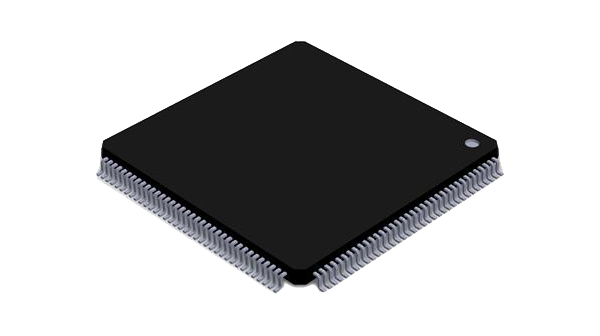
\includegraphics[width=0.6\textwidth]{images/lqfp}
    \caption{LQFP144 microcontroller package}
    \label{fig:LQFP}
\end{figure}

The microcontroller should meet certain parameters to be chosen.
One of the most important parameters is the clock speed.
Digital signal processing requires a lot of processor instructions
per each audio sample, so high clock speed is preferred.

The second important criterion is amount of memory.
The microcontroller should have at least 128kB of ROM
to fit the written program.
Size of RAM should be as high as possible,
because delay effects require a lot of memory.

Presence of FPU is preferred due to its performance benefits.
Dedicated floating-point hardware greatly decreases time
needed for floating-point calculations.

To reduce the total cost of the device,
proper A/D and D/A converters could be included in the microcontroller.

All of above criterion is met by STM32H743ZI microcontroller.
It is based on Arm Cortex-M7 32-bit RISC core.
This specific model uses LQFP144 package.
Most important parameters of this microcontroller are listed below:
\begin{itemize}
    \item 480MHz maximum clock frequency
    \item 1MB of RAM and 2MB of Flash memory
    \item single and double precision FPU and set of DPS instructions
    \item 16-bit ADC and 12-bit DAC
    \item 140 I/Os and selection of peripherals such as hardware
    SPI, I2C, I2S, UART, SPDIF, USB OTG
\end{itemize}

\begin{figure}[H]
    \centering
    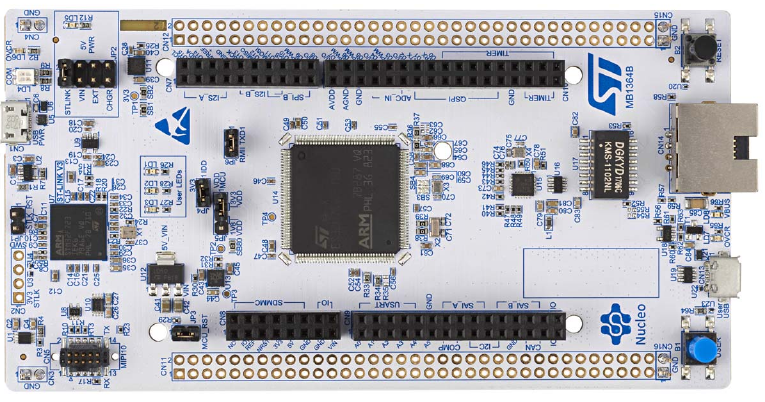
\includegraphics[width=\textwidth]{images/Nucleo}
    \caption{Nucleo H7 development board}
    \label{fig:Nucleo}
\end{figure}

The STM32H743ZI comes one the NUCLEO-H743ZI evaluation board.
It includes ST-LINK debugger/programmer,
which simplified development of the device. 


\subsection {Operational amplifiers}

TLC272C was operational amplifier of choice.
It contains two amplifiers in a single SMD package, which is SOIC-8.
Main constraining factor for choice of this element was power supply.
Analog power supplied on the board is 3.3V, so the operational amplifier
must be capable of operating in such condition.
TLC272C is designed to work with single-supply configuration
and voltages as low as 3V,
while providing 2V of undistorted output voltage swing.

\section{Schematic}

Schematic was created using KiCad EDA,
which is both cross-platform and open source software.
It provides rich library of components and very intuitive user interface.

Schematic is divided into three parts,
each containing component related to each other.
Analog part is devoted to input and output amplifiers.
In digital section we can find external memory, LCD and rotary encoder.
Last part is dedicated to gold pins connecting shield to a Nucleo board.

\begin{figure}[H]
    \centering
    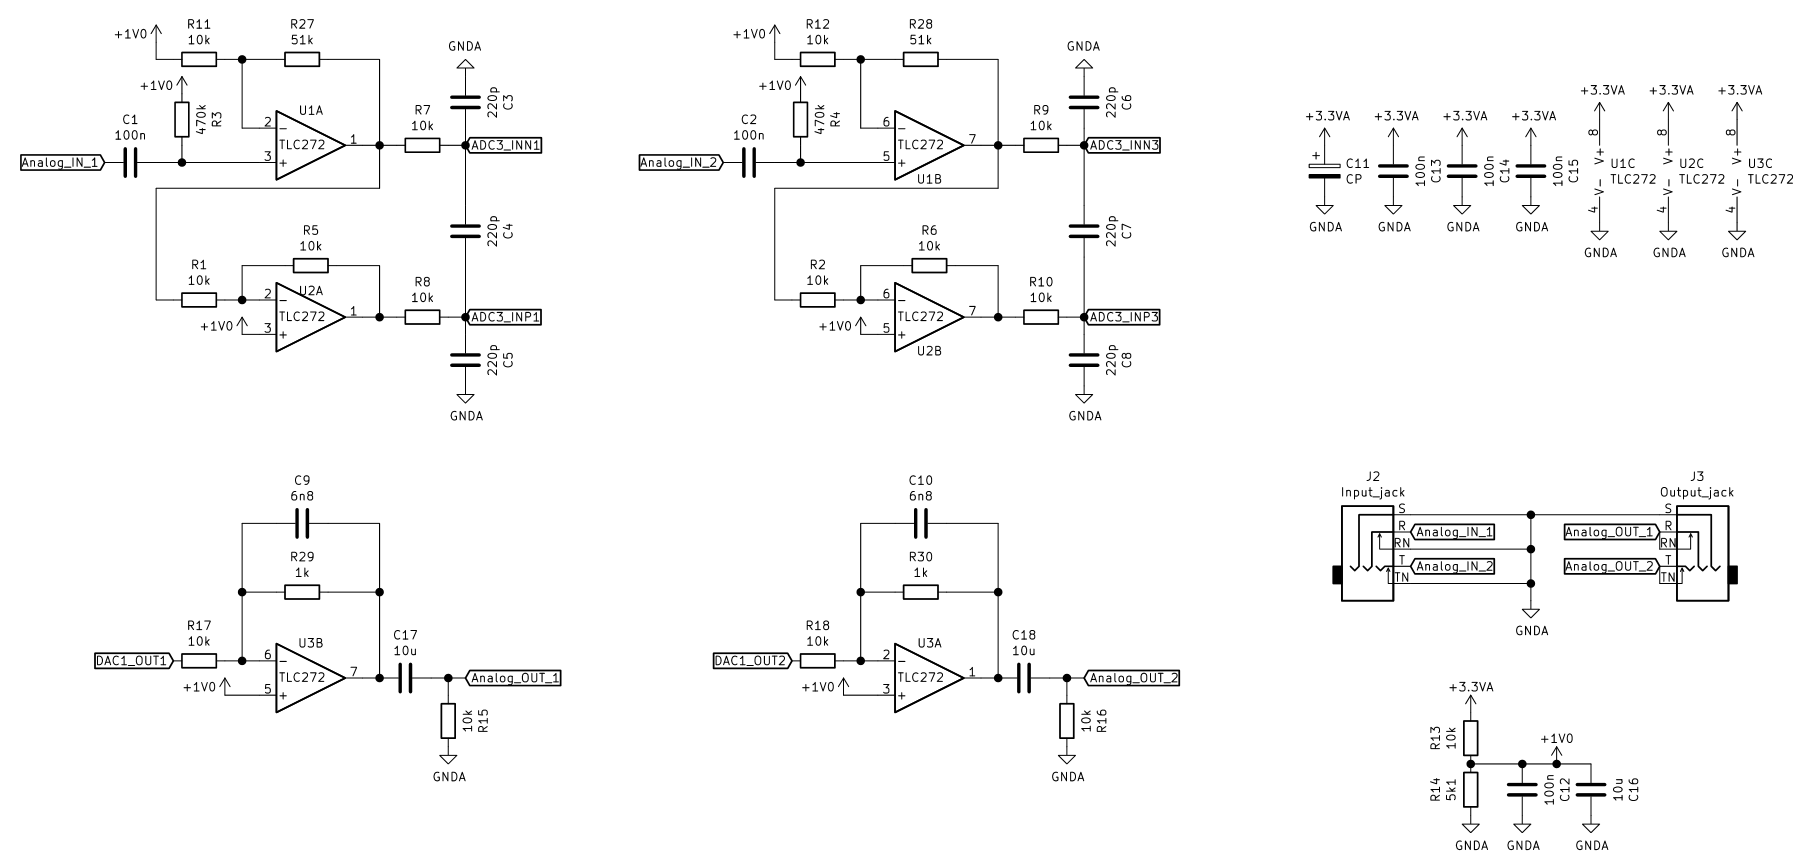
\includegraphics[width=\textwidth]{images/Schematic_analog}
    \caption{Schamatic of analog part of the device}
    \label{fig:Schematic1}
\end{figure}

\begin{figure}[H]
    \centering
    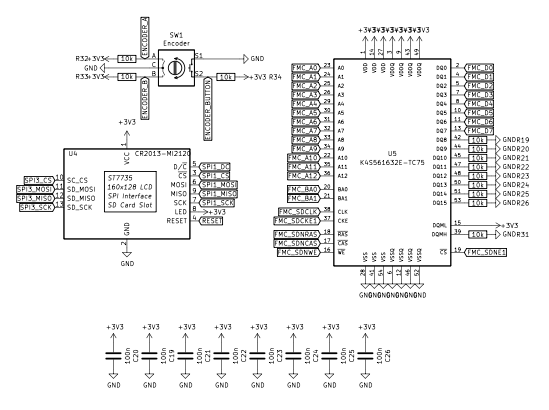
\includegraphics[width=0.8\textwidth]{images/Schematic_digital}
    \caption{Schamatic of digital part of the device}
    \label{fig:Schematic2}
\end{figure}

\begin{figure}[H]
    \centering
    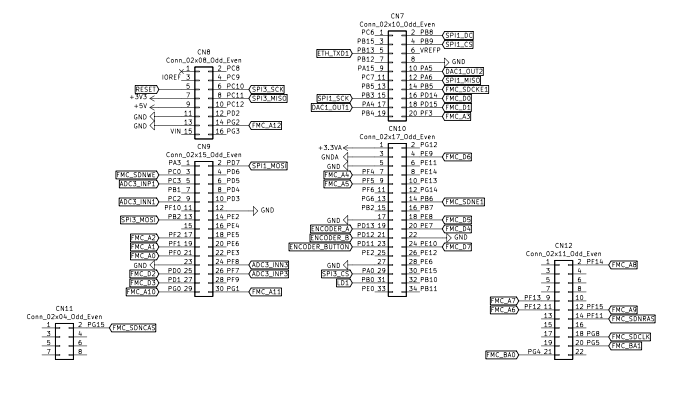
\includegraphics[width=0.8\textwidth]{images/Schematic_connectors}
    \caption{Schamatic of gold pin connectors}
    \label{fig:Schematic3}
\end{figure}

\section{PCB}
PCB layout was prepared using KiCad EDA as well.
All elements except for gold pin headers,
rotary encoder and audio jacks are SMD (surface mounted).
To reduce cost of the project, the PCB was designed as 2 layer board only.
This decision resulted in increased difficulty of routing process.
Gerber files generated by the software were sent to manufacturer in China
and arrived two weeks later.

\begin{figure}[H]
    \centering
    \begin{subfigure}[h]{0.3\textwidth}
        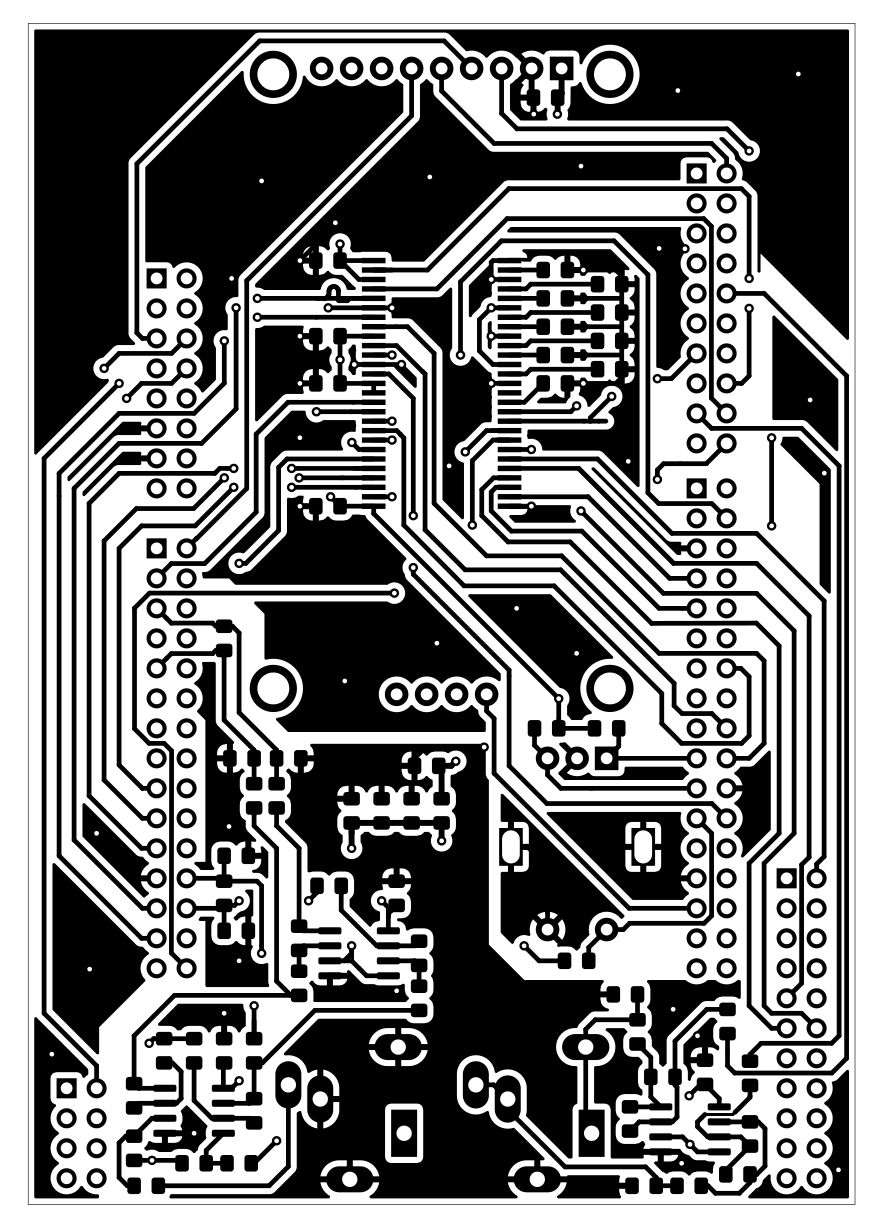
\includegraphics[width=\textwidth]{images/Board_front}
        \label{fig:board1}
        \caption{Front copper}
    \end{subfigure}
    ~
    \begin{subfigure}[h]{0.3\textwidth}
        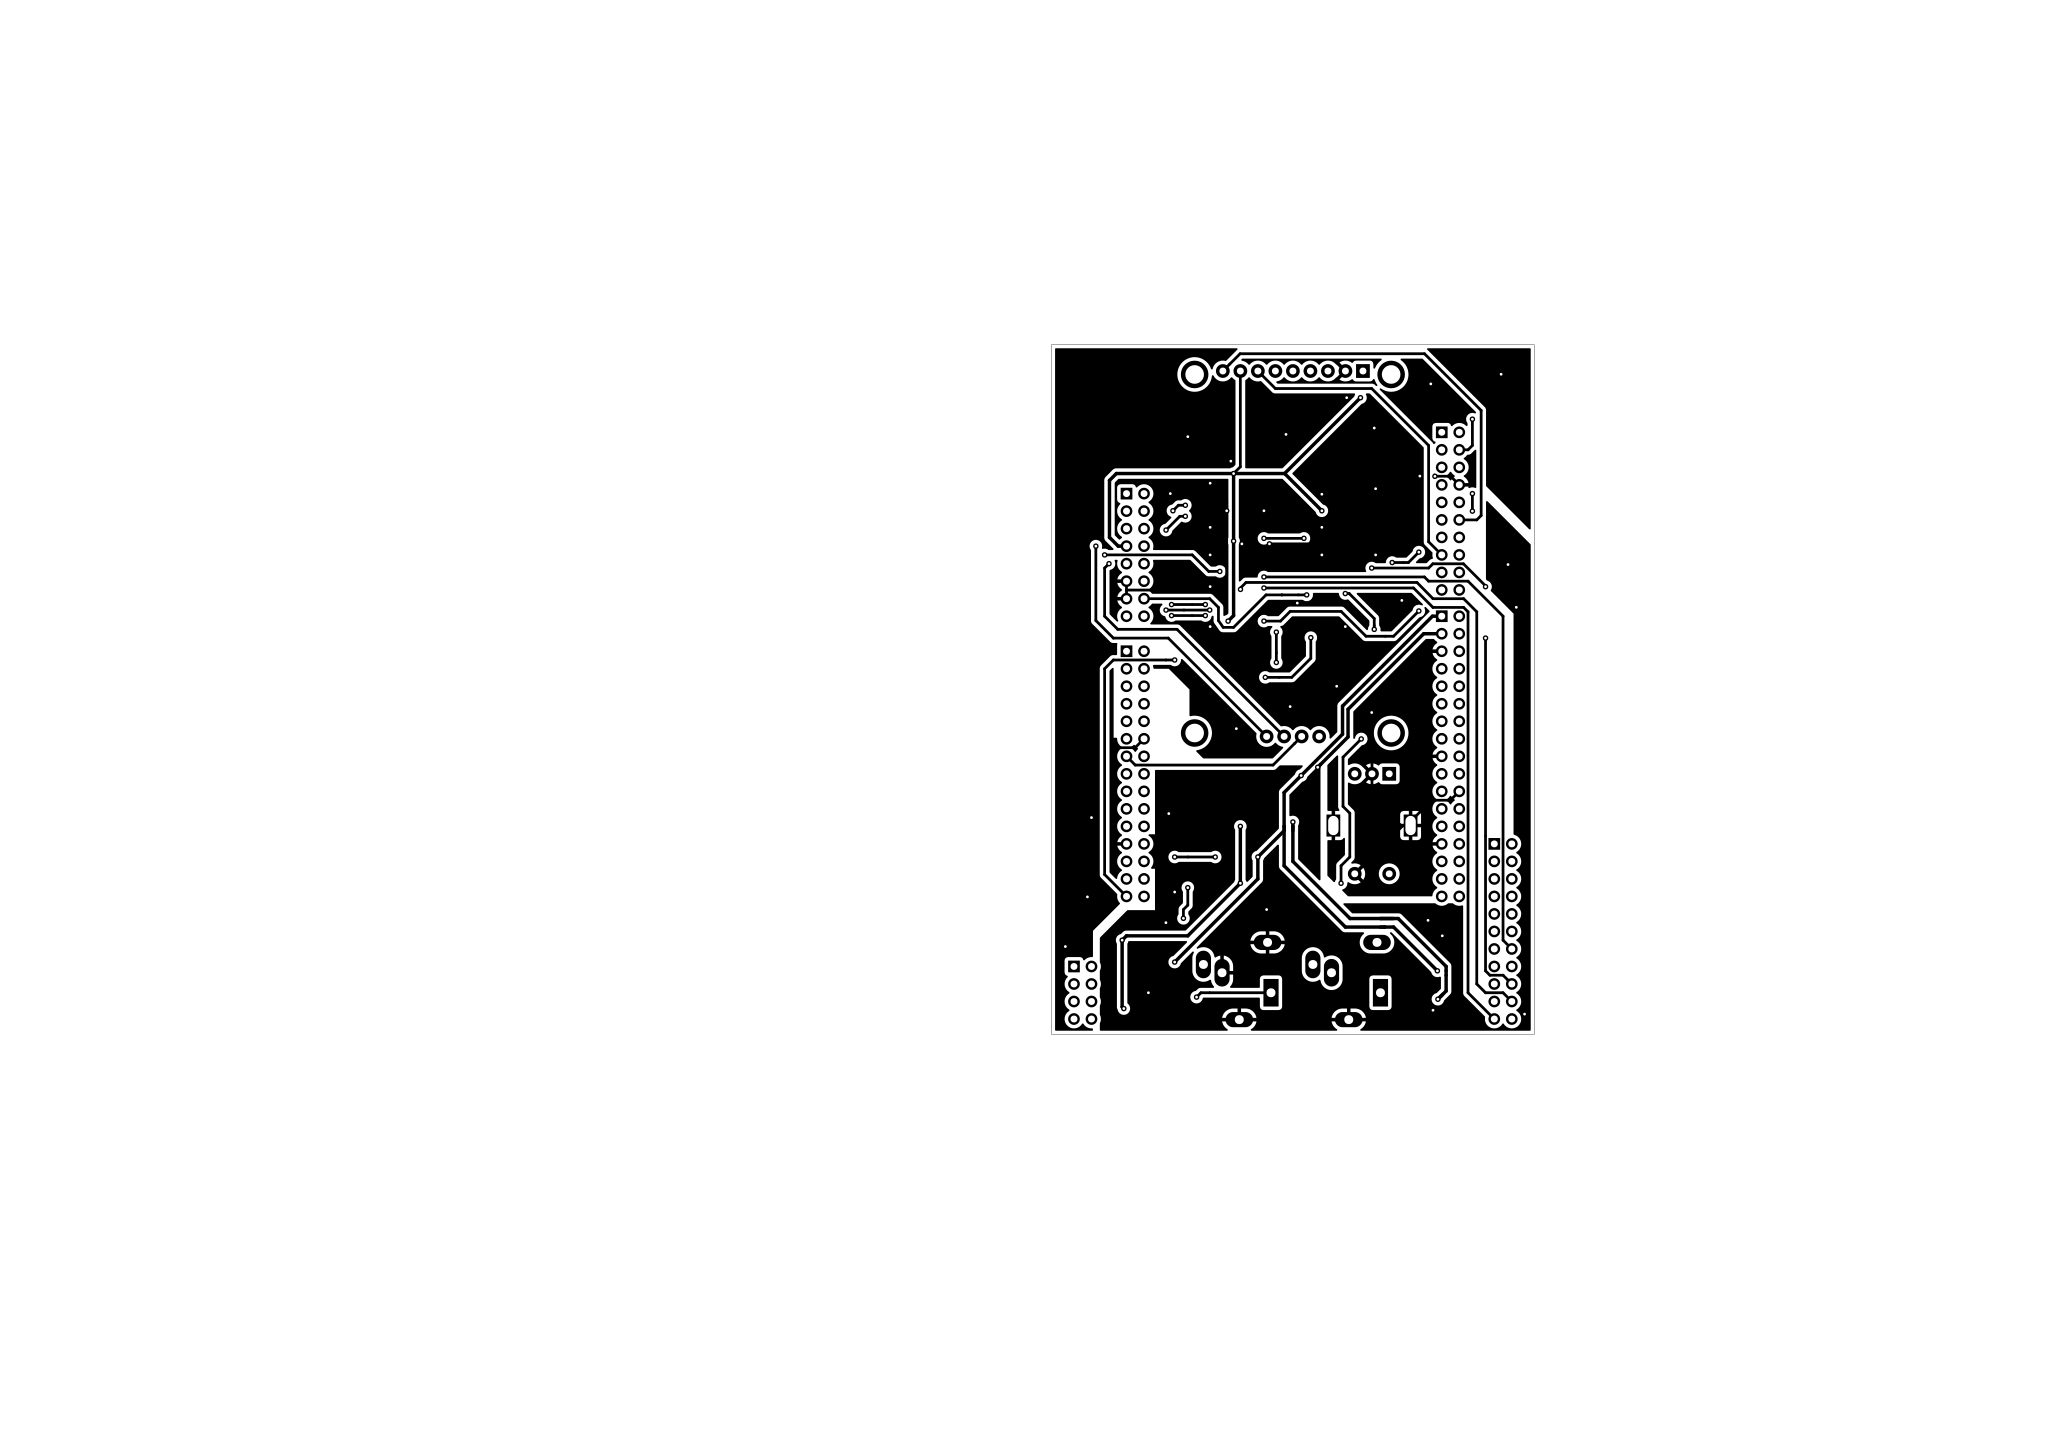
\includegraphics[width=\textwidth]{images/Board_back}
        \label{fig:board2}
        \caption{Back copper}
    \end{subfigure}
    ~
    \begin{subfigure}[h]{0.3\textwidth}
        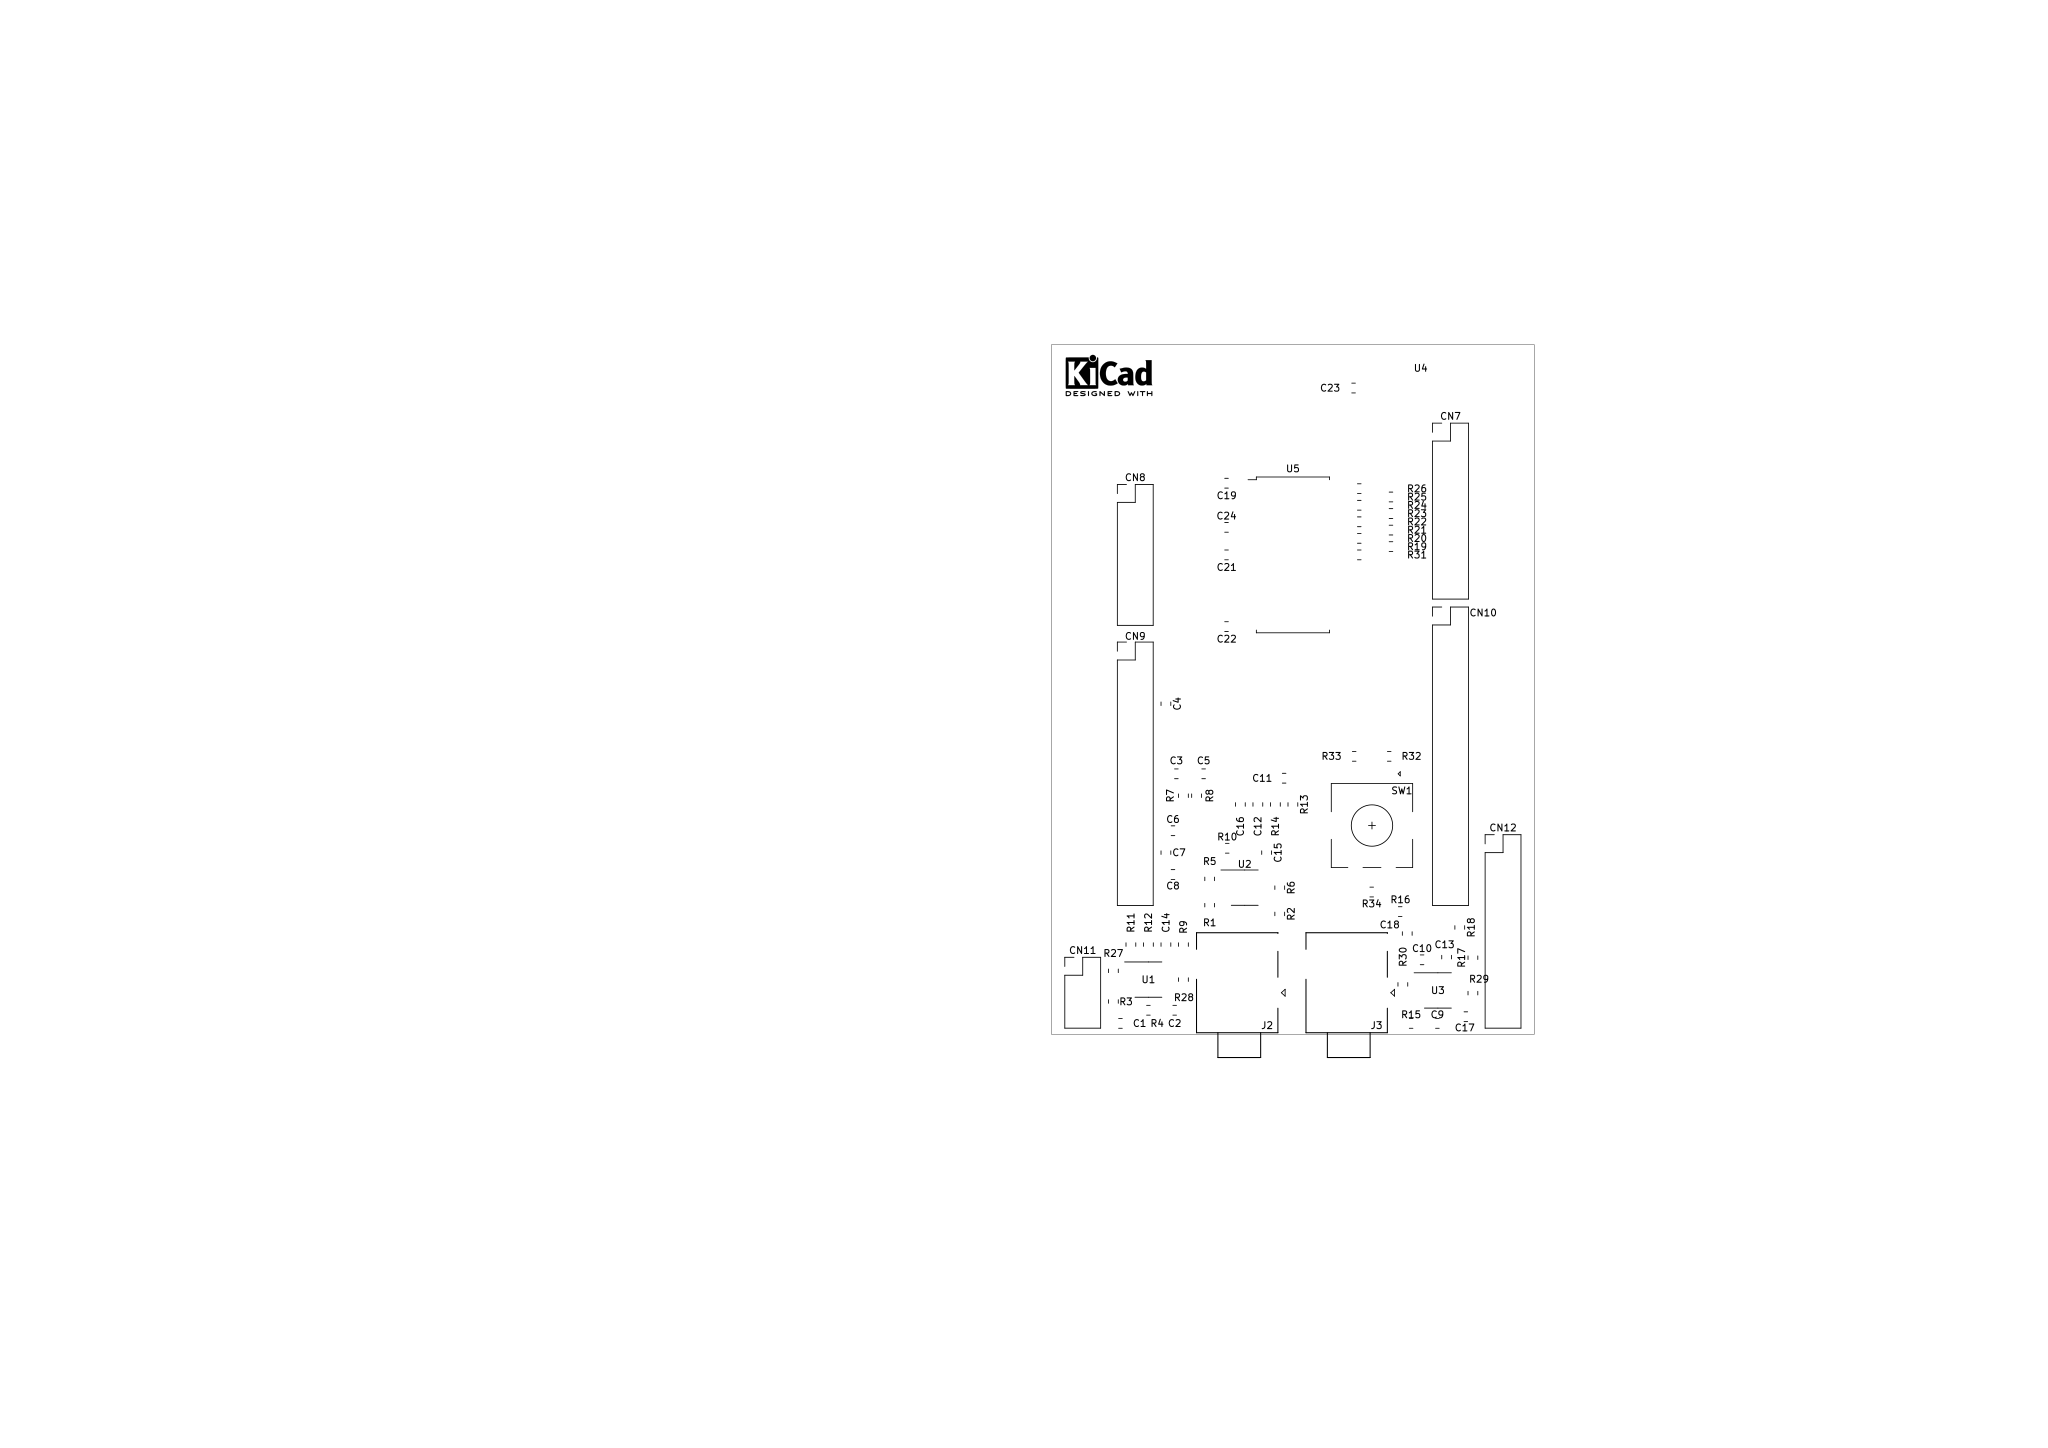
\includegraphics[width=\textwidth]{images/Board_silkscreen}
        \label{fig:board3}
        \caption{Front silkscreen}
    \end{subfigure}
    \caption{Copper and silkscreen layers of the PCB}
    \label{fig:board}
\end{figure}

\begin{figure}[H]
    \centering
    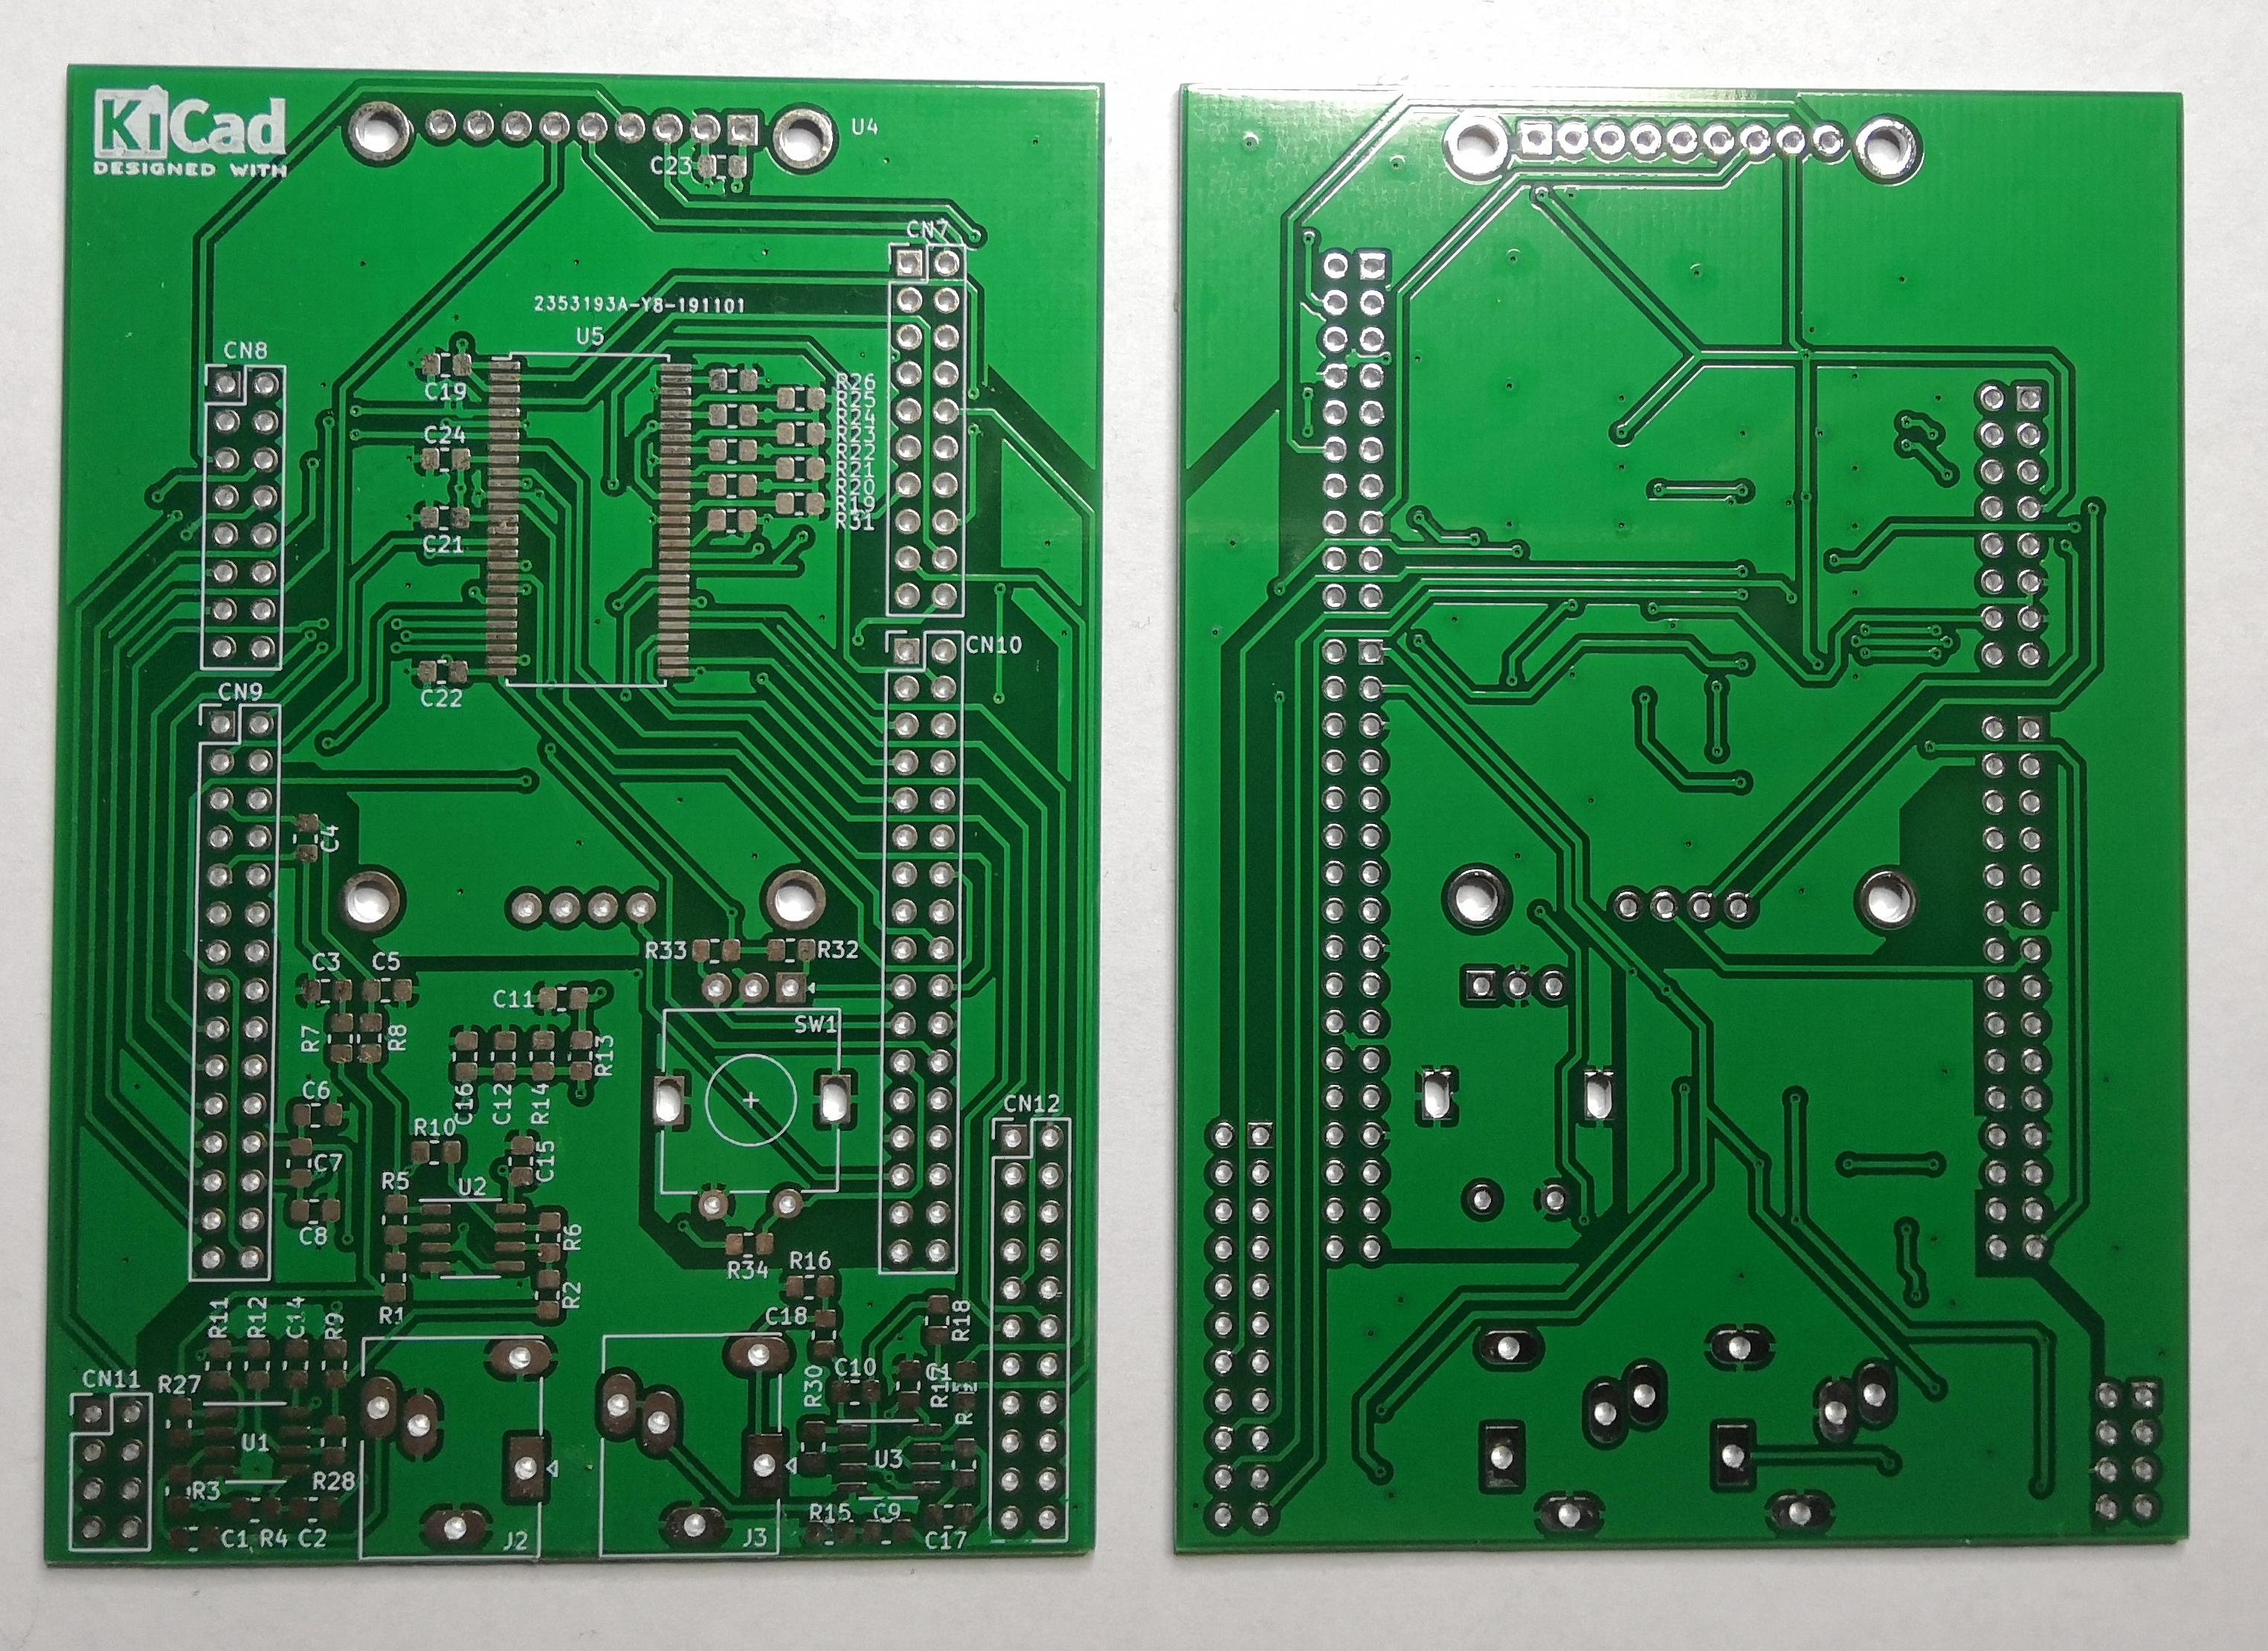
\includegraphics[width=\textwidth]{images/photo_boards}
    \caption{Photo of front and back sides of the PCB}
    \label{fig:photo_boards}
\end{figure}

\section{Assembly}
The PCB was populated by hand using 50W soldering iron and hot air rework station.
Two types of tin-lead solder were used during the process:
0.25mm solder wire (Sn60 Pb40) for THT components and solder paste (Sn62 Pb36 Ag2) for SMD.

\begin{figure}[H]
    \centering
    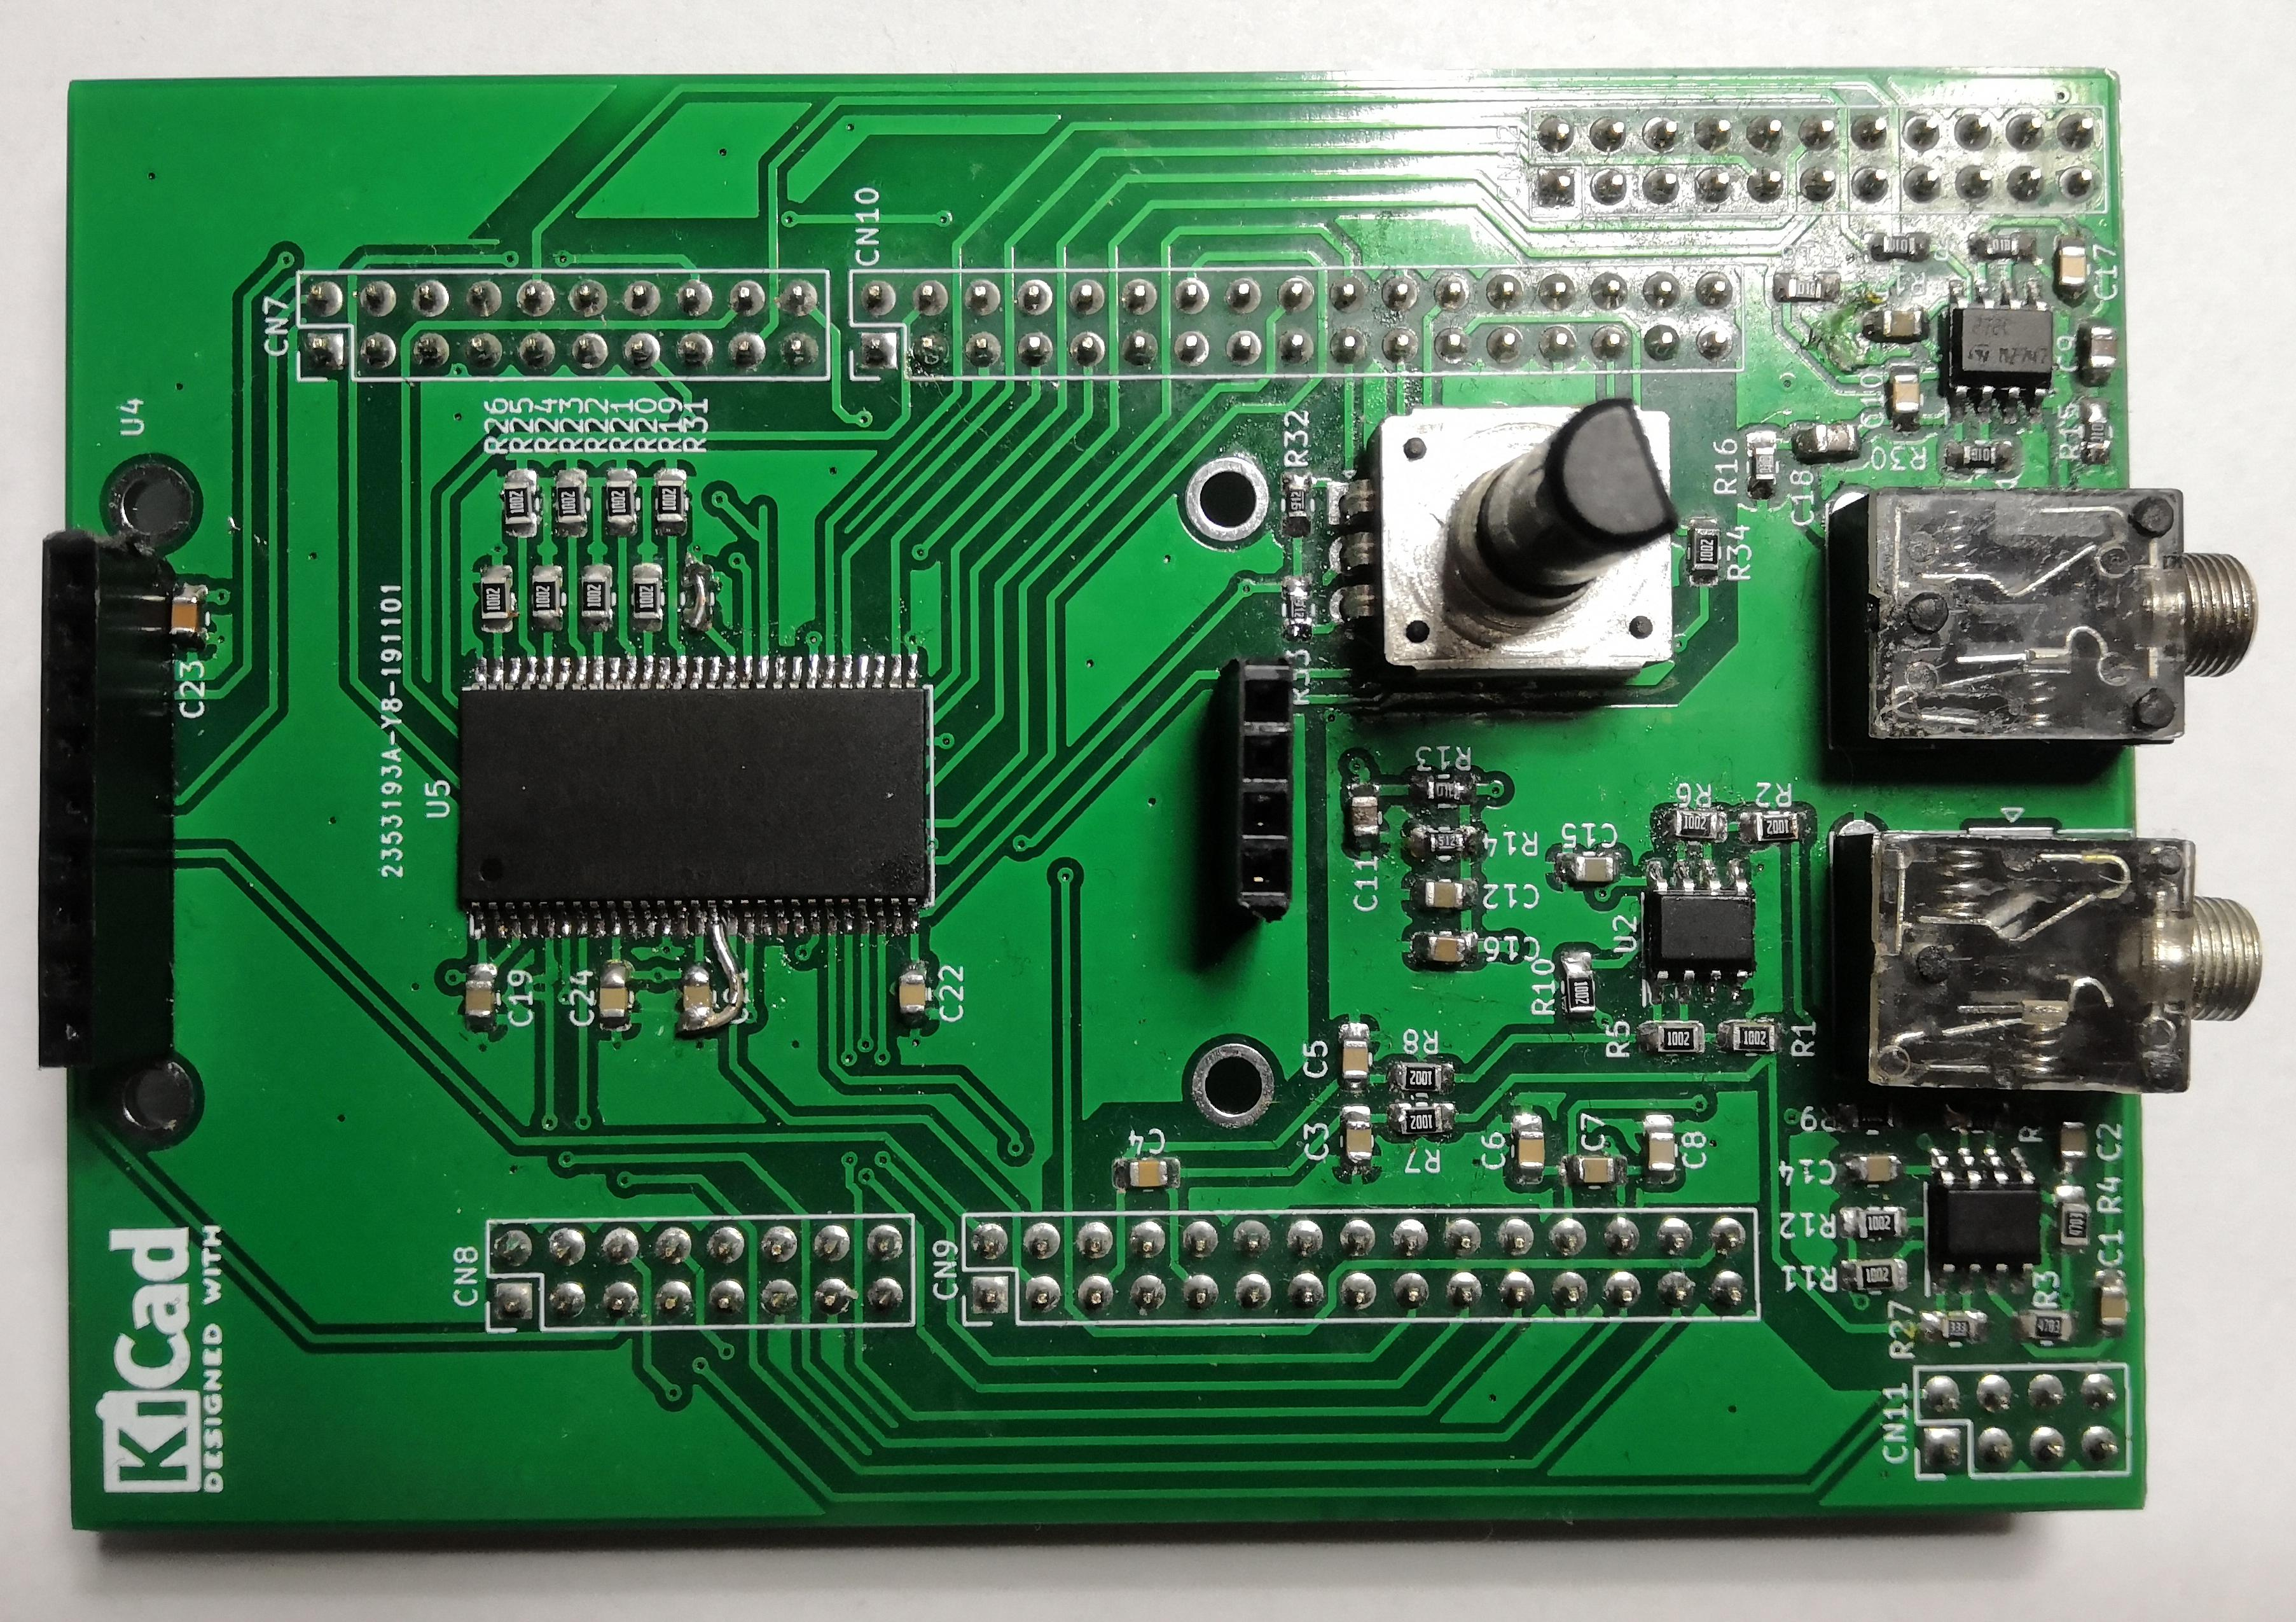
\includegraphics[width=\textwidth]{images/photo_assembled}
    \caption{Photo of assembled board}
    \label{fig:pgoto_assembled}
\end{figure}



\chapter{Internal specification}

\section{Programming environment}
Programming environment consist of several tools,
that need to work together to facilitate software development.
All tools used in this project are cross-platform.
Following section is devoted to choice of these tools.

\subsection{Programming language}

\begin{figure}[H]
    \centering
    \begin{subfigure}[h]{0.3\textwidth}
        
\includegraphics[width=\textwidth]{images/c_logo}
        \label{fig:c}
    \end{subfigure}
    ~
    \begin{subfigure}[h]{0.3\textwidth}
        
\includegraphics[width=\textwidth]{images/cpp_logo}
        \label{fig:cpp}
    \end{subfigure}
    \caption{C and C++ languages logos}
    \label{fig:lang}
\end{figure}

C language is the most popular choice for STM32 development.
It is widely supported by ST and other companies providing frameworks and libraries.
As a low level language, it provides control over memory management,
which is a important factor in software development for microcontrollers.

Since the object oriented approach was preferred in this project,
C++ language was chosen.
This allows to benefit from libraries written in C,
but also gives advantages of using classes with inheritance and polymorphism,
which are part of C++ language.

\subsection{IDE}

\begin{figure}[H]
    \centering
    
\includegraphics[width=0.3\textwidth]{images/platformio-logo}
    \caption{PlatformIO IDE logo}
    \label{fig:plaftormio}
\end{figure}

The popular environments for STM32 development are Keil uVision, IAR and SW4STM32.
ST also provides its own STM32CubeIDE, which is based on Eclipse.

Another choice is PlatformIO IDE.
It is free and open source IDE and
comes as a plugin for Visual Studio Code and Atom text editors.
It provides all libraries, frameworks,
debugger server and compiler necessary for STM32 software development.

\subsection{Text editor}
\begin{figure}[H]
    \centering
    
\includegraphics[width=0.3\textwidth]{images/vscode}
    \caption{Visual Studio Code logo}
    \label{fig:vscode}
\end{figure}

Visual Studio Code is a free code editor developed by Microsoft.
It was chosen because it is supported by PlatformIO IDE.
VSCode provides linting and word completion extensions,
which simplify the process of software development.

\subsection{Frameworks and tools}

\begin{figure}[H]
    \centering
    \begin{subfigure}[h]{0.3\textwidth}
        
\includegraphics[width=\textwidth]{images/cube_logo}
        \label{fig:cube}
    \end{subfigure}
    ~
    \begin{subfigure}[h]{0.3\textwidth}
        
\includegraphics[width=\textwidth]{images/arm_logo}
        \label{fig:arm}
    \end{subfigure}
    ~
    \begin{subfigure}[h]{0.3\textwidth}
        
\includegraphics[width=\textwidth]{images/gnu_logo}
        \label{fig:gnu}
    \end{subfigure}
    \caption{Logos of SMT32Cube, Arm and the GNU project}
    \label{fig:tools}
\end{figure}

List of frameworks and additional tools used for software development:

\begin{itemize}
    \item HAL drivers
    - Hardware Abstraction Layer driver is a library written in C language, provided by ST.
    It allows an easy use of microcontroller and code compatibility between different STM32 devices.
    \item STM32CubeMX
    - a graphical tool that allows an easy STM32 configuration.
    It generates configuration code for the microcontroller and desired peripherals in C language.
    STM32CubeMX uses HAL driver in generated initialization code.
    \item CMSIS
    - Cortex Microcontroller Software Interface Standard
    is a hardware abstraction layer provided by Arm.
    It is compatible with all Arm Cortex microprocessors and microcontrollers.
    It includes API for Cortex-M and Cortex-A core and peripherals as well as additional tools
    (DSP library, neural network kernels, real-time operating systems).
    \item OpenOCD
    - Open On-Chip Debugger provides programming and debugging support of boundary scan interface.
    It supports ST-Link, which was used for both programming and debugging of STM32 microcontroller.
    \item GNU Embedded Toolchain for Arm
    is a suite of tools for C, C++ and Assembly programming provided and maintained by Arm.
    It contains the GCC Compiler as well as linker.
\end{itemize}

\section{Software block diagram}
\cite{ST:UM2407}

\section{Configuration}

\begin{figure}[H]
    \centering
    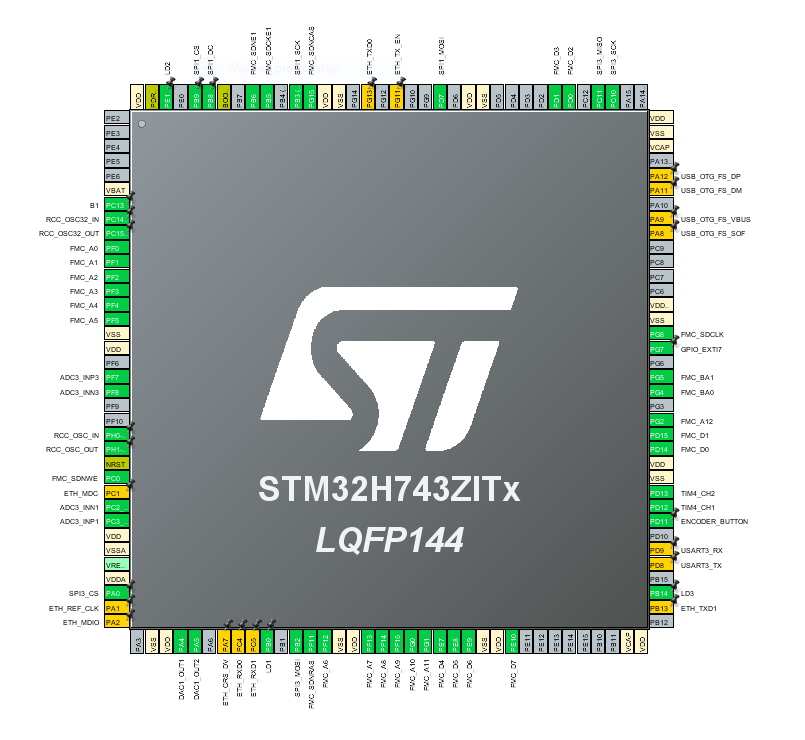
\includegraphics[width=\textwidth]{images/pin_overview}
    \caption{Screenshot of the pin configuration in STM32CubeMX software}
    \label{fig:pins}
\end{figure}

\begin{itemize}
    \item Code generation

    Initialization code was generated using STM32CubeMX software.
    It provided necessery implementation of initialization functions
    as well as general structure of the program.
    Each enabled peripheral has its own source file
    and corresponding header file.

    \item Clock

    Maximum clock frequency for this version of MCU is 400MHz.
    Unfortunately it is not divisible by 48kHz, which is our sampling frequency.
    For that reason clock prescalers are set to obtain 396MHz clock frequency.
    This way it is easy to setup desired sampling frequency on one of the timers.
    Clock was also configured using STM32CubeMX software.

    \item Environmental settings
    
    All settings passed to tools such as linter, compiler and linker
    are present in platformio.ini and extra\_script.py files.
    These settings give information about used frameworks
    and paths to specific libraries and header files.

    \begin{figure}[H]
    \centering
    \begin{lstlisting}
    [platformio]
    include_dir = ./Inc

    [env:nucleo_h743zi]
    platform = ststm32
    board = nucleo_h743zi
    framework = stm32cube
    board_build.f_cpu = 396000000L
    board_upload.maximum_ram_size = 65536
    build_flags =   -I ${PROJECT_PACKAGES_DIR}/framework-stm32cube/h7/Drivers/CMSIS/DSP/Include
                    -I ${PROJECT_PACKAGES_DIR}/framework-stm32cube/h7/Drivers/STM32H7xx_HAL_Driver/Inc
                    -L ${PROJECT_PACKAGES_DIR}/framework-stm32cube/h7/Drivers/CMSIS/Lib/GCC
                    -l libarm_cortexM7lfsp_math.a
                    -D ARM_MATH_CM7
                    -D __FPU_PRESENT=1
    extra_scripts = pre:extra_script.py
    \end{lstlisting}
    \caption{Contentes of platformio.ini file}
    \label{fig:ini}
    \end{figure}

    \item FPU

    Floating-point unit present in the microcontroller must be enabled
    using special compiler flags. Without them program would be compiled
    using software floating-point, which is very slow and unefficient.
    -mfpu=fpv5-d16 flag specifies version of arm FPU present in microcontroller.
    -mfloat-abi=hard forces to compile with hardware floating-point.
    Both of them are set in extra\_script.py file.

    \item Cache
    
    STM32H7 series of microcontrollers provide both data and instruction cache.
    This kind of memory can enhance performance of the device,
    since it is twice as fast as other sections of RAM.
    Despite the performance gain, cache (especially data cache)
    must be used with caution, since it can cause some issues with DMA.
    The solution involves using cache clear and invalidation functions.
    These function forces transfer between RAM and cache in order to ensue,
    that DMA is referencing valid data.

    \item Memory organization
    \begin{figure}[H]
    \centering
    \begin{lstlisting}
/* Specify the memory areas */
MEMORY
{
ITCMRAM (xrw)   : ORIGIN = 0x00000000, LENGTH = 64K
FLASH (rx)      : ORIGIN = 0x08000000, LENGTH = 2048K
DTCMRAM (xrw)   : ORIGIN = 0x20000000, LENGTH = 128K
RAM_D1 (xrw)    : ORIGIN = 0x24000000, LENGTH = 512K
RAM_D2 (xrw)    : ORIGIN = 0x30000000, LENGTH = 288K
RAM_D3 (xrw)    : ORIGIN = 0x38000000, LENGTH = 64K
SDRAM (xrw)     : ORIGIN = 0xD0000000, LENGTH = 16M
}
    \end{lstlisting}
    \caption{Memory layout from linker script.}
    \label{fig:mem}
    \end{figure}

    \item ADC
    
    ADC is set to continuous conversion mode.
    It is constatnly converting signal with sampling rate above 100kHz.
    Obtained samples are than transfered to a buffer using DMA.
    Parallel to ADC, a timer is generating interrupts
    with rate equal 48kHz. During such interrupt,
    freshest sample is copied into block buffers. 
    When the block buffer is full, it can be swaped with empty buffer
    and than processed.

    \item DAC
    \item Timer
    \item SPI

\end{itemize}

\section{Description of functions and objects}

\begin{itemize}
    \item Global variables and constants
    \begin{figure}[H]
    \centering
    \begin{lstlisting}
/* USER CODE BEGIN Private defines */
#define BLOCK_SIZE 512
#define SAMPLING_RATE 48000
#define NO_OF_CHANNELS 2
#define ADC_RESOLUTION 16
#define DELAY_SIZE (SAMPLING_RATE + BLOCK_SIZE) // 1s + block size
#define MODULATION_DELAY_SIZE (2 * 1440 + BLOCK_SIZE) // 30ms + block size
/* USER CODE END Private defines */
    \end{lstlisting}
    \caption{Global defines from main.h file.}
    \label{fig:defs}
    \end{figure}

    \begin{figure}[H]
    \centering
    \begin{lstlisting}
/* USER CODE BEGIN PD */
#define AXI_SRAM_D1 __attribute__((section(".axi_sram_d1")))
#define AHB_SRAM_D2 __attribute__((section(".ahb_sram_d2")))
#define ALIGN_32 __attribute__((aligned(0x20)))
/* USER CODE END PD */

// Global flags
uint16_t block_counter = 0;
uint8_t block_ready = 0;

// Allocation in different parts of memory
float32_t AXI_SRAM_D1 delay_buffer1[DELAY_SIZE];
float32_t AXI_SRAM_D1 delay_buffer2[DELAY_SIZE];
float32_t AXI_SRAM_D1 mod_buffer1[MODULATION_DELAY_SIZE];
float32_t AXI_SRAM_D1 mod_buffer2[MODULATION_DELAY_SIZE];
uint8_t AHB_SRAM_D2 ALIGN_32 character_buffer[128];
uint32_t AHB_SRAM_D2 ALIGN_32 input_sample[2];

// Defining global buffers
uint16_t buffer[6][BLOCK_SIZE];
uint16_t *input_buffer = buffer[0];
uint16_t *hidden_buffer = buffer[2];
uint16_t *output_buffer = buffer[4];
    \end{lstlisting}
    \caption{Global variables from main.cpp file.}
    \label{fig:vars}
    \end{figure}

    \item Main loop
    \begin{figure}[H]
    \centering
    \begin{lstlisting}
while (true) {
  if (block_ready) {
    HAL_GPIO_WritePin(LD3_GPIO_Port, LD3_Pin, GPIO_PIN_SET);

    // Convert data to float
    arm_uint16_to_float(&hidden_buffer[0], &data[0][0], BLOCK_SIZE);
    arm_uint16_to_float(&hidden_buffer[BLOCK_SIZE], &data[1][0], BLOCK_SIZE);

    // Process block of data
    master->ProcessBlock(data[0], data[1], BLOCK_SIZE);
    master->UpdateUI();

    // Convert data back to 16 bit unsigned integer
    arm_float_to_uint16(&data[0][0], &hidden_buffer[0], BLOCK_SIZE);
    arm_float_to_uint16(&data[1][0], &hidden_buffer[BLOCK_SIZE], BLOCK_SIZE);

    // Resetting block rady flag
    block_ready = 0;

    HAL_GPIO_WritePin(LD3_GPIO_Port, LD3_Pin, GPIO_PIN_RESET);
  }

  // Display the next character if DMA is ready for next transfer
  if(HAL_SPI_GetState(&hspi1) == HAL_SPI_STATE_READY){
    master->DisplayPop();
  }
}
    \end{lstlisting}
    \caption{Main loop code.}
    \label{fig:loop}
    \end{figure}

    \item Timer interrupt
    \begin{figure}[H]
    \centering
    \begin{lstlisting}
void HAL_TIM_PeriodElapsedCallback(TIM_HandleTypeDef *htim){
  if(htim->Instance == TIM2){
    // Reading samples from input to buffer
    SCB_InvalidateDCache_by_Addr(input_sample, 32);
    input_buffer[block_counter] = (uint16_t)input_sample[0];
    input_buffer[block_counter+BLOCK_SIZE] = (uint16_t)input_sample[1];

    // Writing samples to output
    HAL_DAC_SetValue(&hdac1, DAC1_CHANNEL_1, DAC_ALIGN_12B_R, output_buffer[block_counter]>>4);
    HAL_DAC_SetValue(&hdac1, DAC1_CHANNEL_2, DAC_ALIGN_12B_R, output_buffer[block_counter+BLOCK_SIZE]>>4);

    block_counter++;
    if (block_counter >= BLOCK_SIZE){
      // Swapping buffers
      uint16_t* temp = output_buffer;
      output_buffer = hidden_buffer;
      hidden_buffer = input_buffer;
      input_buffer = temp;
      block_counter = 0;
      block_ready = 1;
    }
  }
}
    \end{lstlisting}
    \caption{Timer interrupt code.}
    \label{fig:timer}
    \end{figure}

    \item Effect class
    \begin{figure}[H]
    \centering
    \begin{lstlisting}
class Effect {
   protected:
    char name[9];
    Effect *pNext;
    Effect *pPrev;
    friend class MultiEffect;

   public:
    Parameter *parameters[10];
    uint8_t number_of_parameters;
    int8_t current_parameter;

    Effect();
    ~Effect();
    virtual void ProcessBlock(float32_t *pData_left, float32_t *pData_right, uint32_t block_size) = 0;
    virtual void UpdateParameters() = 0;
    char *GetName();
    char *GetParamName(int8_t param_id);
    char *GetParamValRepr(int8_t param_id);
    Parameter *GetCurrentParam();
    void SetName(const char *name);
};
    \end{lstlisting}
    \caption{Effect class prototype.}
    \label{fig:Effect}
    \end{figure}

    \item Parameter class
    \begin{figure}[H]
    \centering
    \begin{lstlisting}
class Parameter {
   private:
    char name[10];
    char val_repr[6];
    char unit[3];
    int32_t value, min, max, step;
    friend class Effect;

   public:
    Parameter(const char *name, const char *unit, int32_t min, int32_t max, int32_t step, int32_t initial);
    void SetName(const char *name);
    void SetUnit(const char *unit);
    void SetValue(int32_t value);
    int32_t GetValue();
    int32_t GetMin();
    int32_t GetMax();
    int32_t GetStep();
    char *GetName();
    char *GetValRepr();
    void UpdateValRepr();
    void UpdateValue();
};
    \end{lstlisting}
    \caption{Parameter class prototype.}
    \label{fig:Param}
    \end{figure}

    \item MultiEffect class
    \begin{figure}[H]
    \centering
    \begin{lstlisting}
class MultiEffect {
   private:
    Display *my_disp;
    Effect *current_effect, *pHead, *pTail;
    VU *VU_pre_L, *VU_pre_R, *VU_post_L, *VU_post_R;
    TIM_HandleTypeDef *htim;
    uint8_t param_flag = 1;
    uint8_t val_flag = 0;
    uint8_t button_states = 0;
    uint8_t button_pressed = 0;
    uint16_t last_tim_cnt = 0x7FFF;

    void InitializeLCD(SPI_HandleTypeDef *hspi);
    void InitializeEffects();

   public:
    MultiEffect(TIM_HandleTypeDef *encoder_timer, SPI_HandleTypeDef *tft_spi);
    void ProcessBlock(float32_t *pData_left, float32_t *pData_right, uint32_t block_size);
    void UpdateUI();
    float32_t UpdateEncoder(TIM_HandleTypeDef *htim, float32_t var, float32_t min, float32_t max, float32_t step);
    uint8_t UpdateEncoder(TIM_HandleTypeDef *htim);
    void DisplayPop();
    void AddEffect(Effect *pNew);
};
    \end{lstlisting}
    \caption{MultiEffect class prototype.}
    \label{fig:Multi}
    \end{figure}
\end{itemize}


\section{User manual}

\begin{figure}[H]
    \centering
    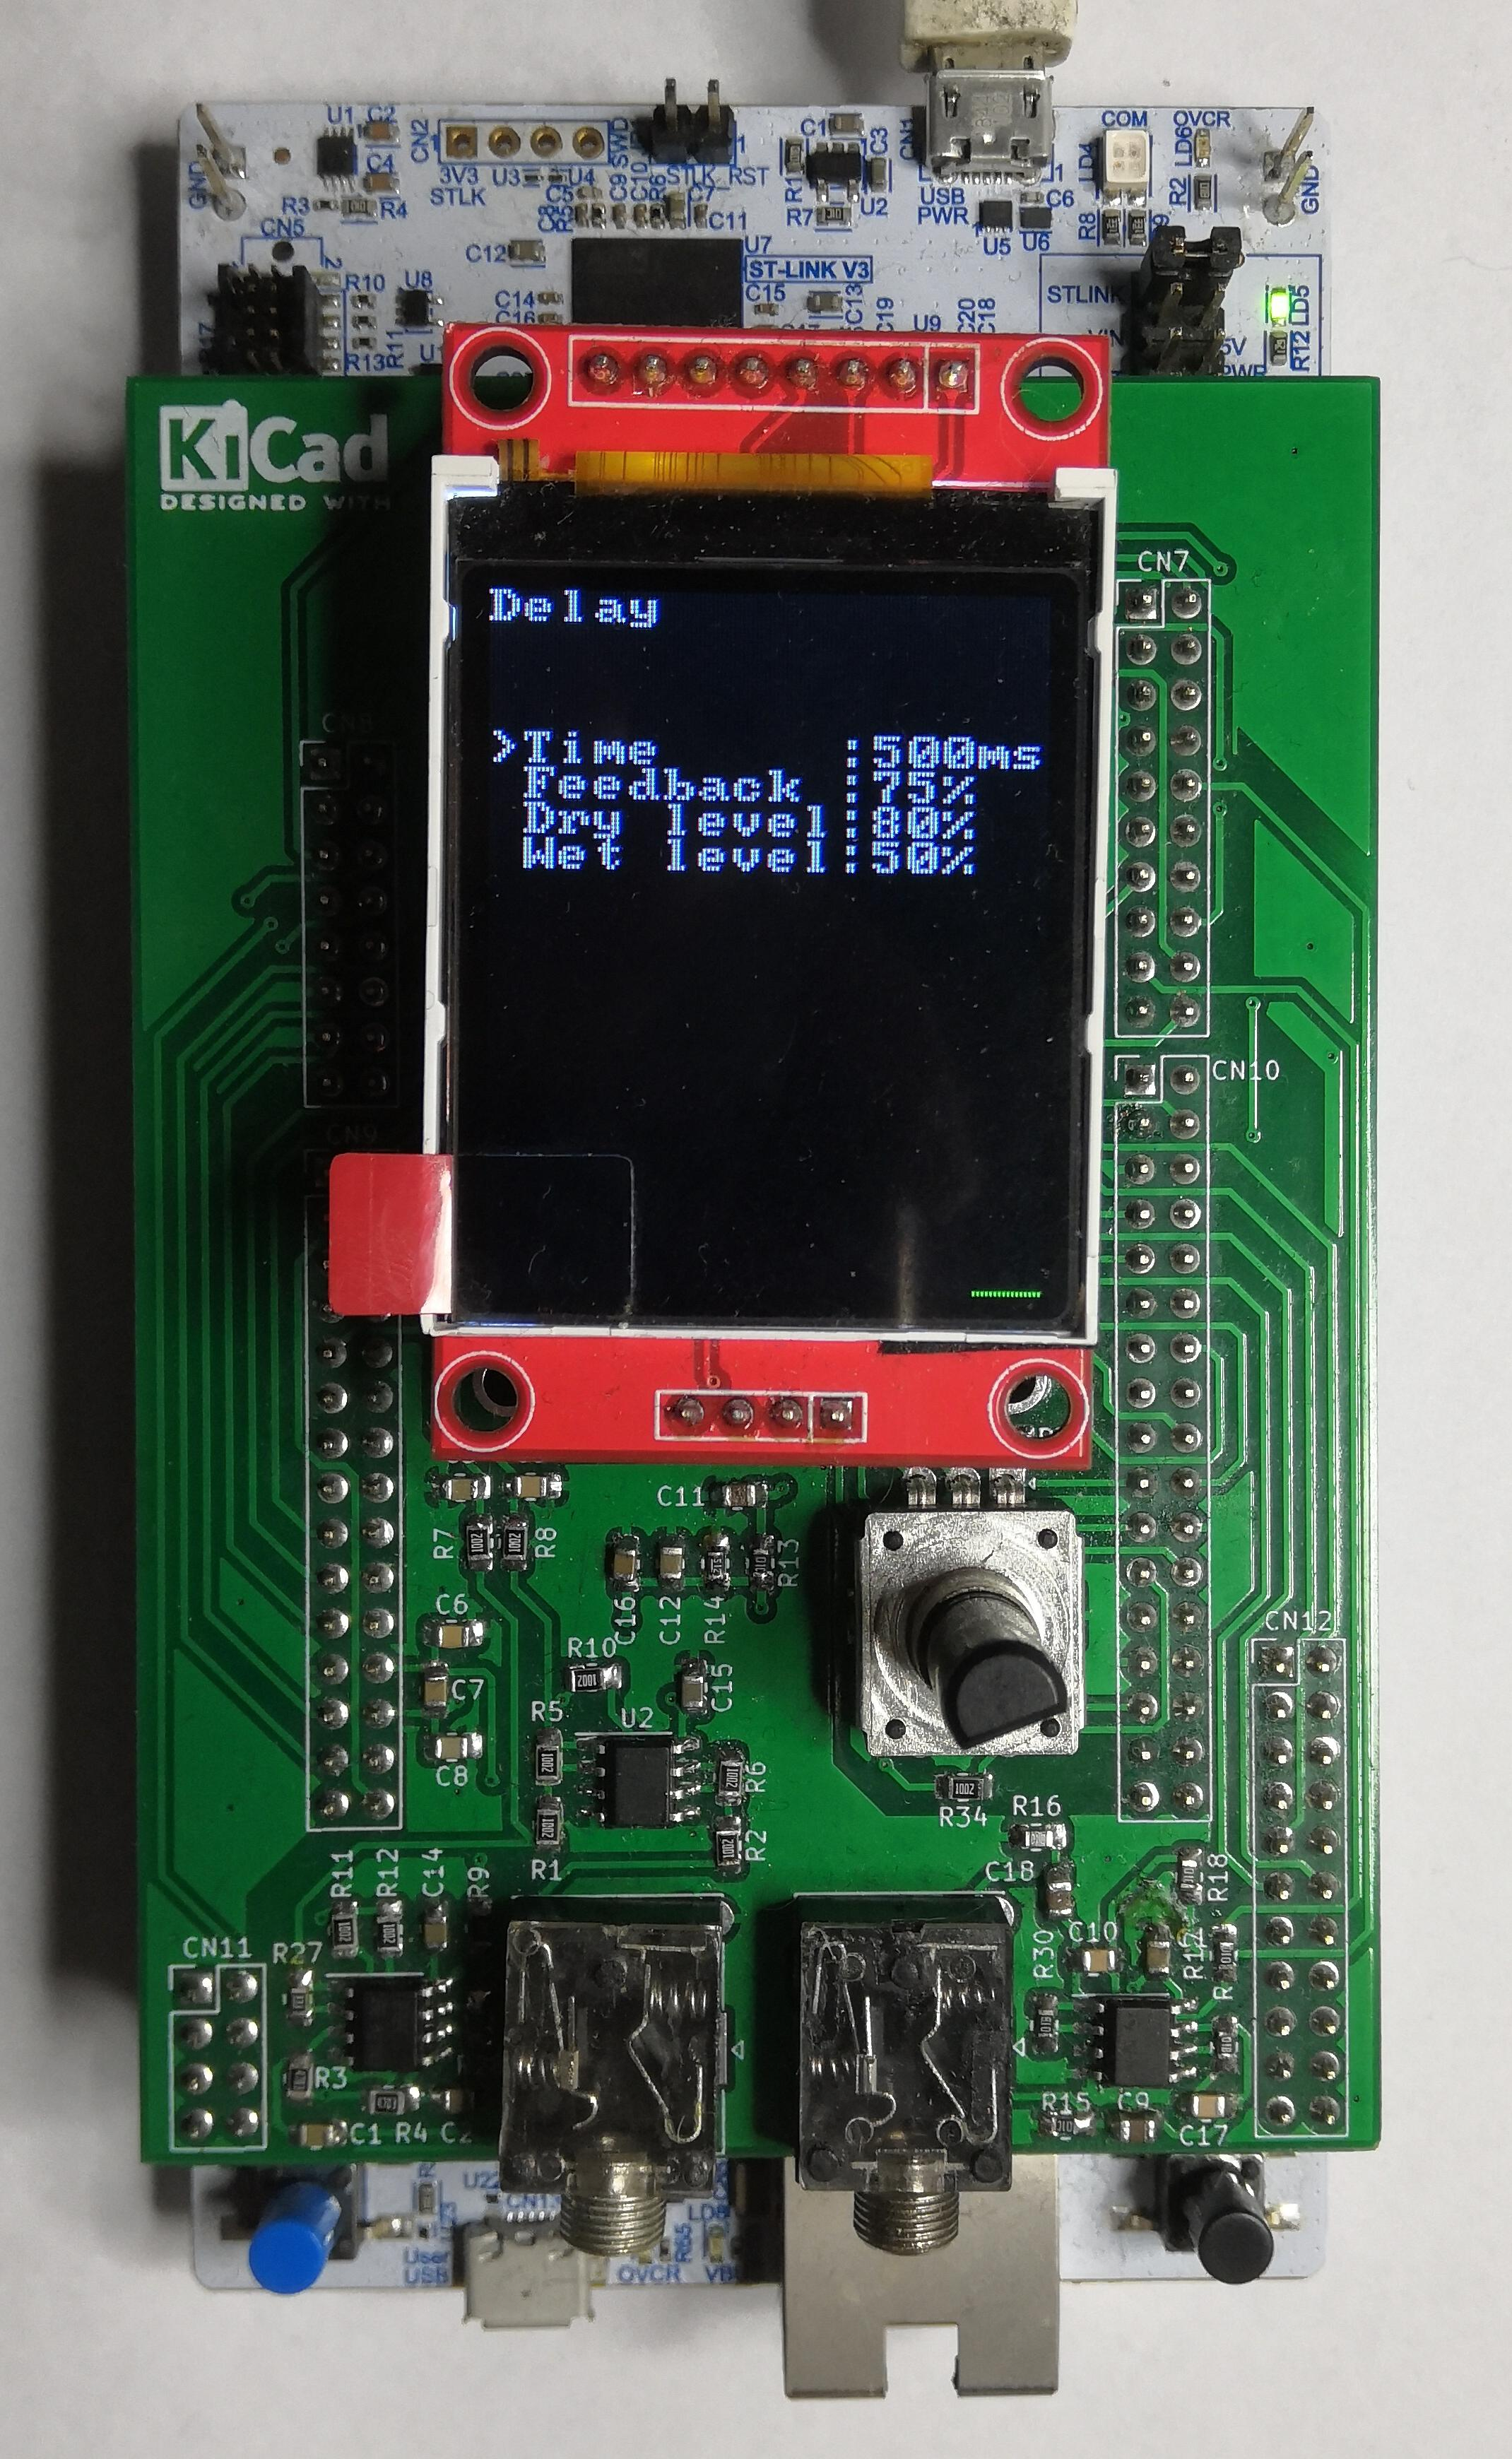
\includegraphics[width=0.5\textwidth]{images/photo_working}
    \caption{Photo of the device during operation}
    \label{fig:working}
\end{figure}

To use the device it must be connected to a power source.
It requires 5V to be applied through the top USB port,
which can be provided by micro USB smartphone charger,
powerbank or directly from computer.

The device has two mini jack connectors on the bottom of the board.
Connector on the left is analog output for the signal source.
It can be connected to line output of smartphone or computer sound card.
Right connector is analog output and should be connected
to an audio amplifier or active speakers.

While powered, the LCD screen should light up
and display white text on black background.
In the left top corner, name of currently selected effect is presented.
Below we can see a list of all parameters,
which can affect behavior of the effect.
On the right of each parameter, there is presented its current value.
On the left side, there is an arrow,
which purpose is to indicate currently selected parameter.

User can interract with device using rotary encoder
as well as black and blue buttons.
Rotating knob changes currently selected parameter.
To modify value of chosen parameter, user must push the encoder
to activate edit mode. It is indicated by green color of text.
In edit mode use can rotate knob to modify chosen value
and press it one more time to accept changes.

To change active effect, user must rotate the encoder
while blue button is depressed. User can also reset the device if needed.
To do it, user can press the black button,
which a hardware reset for both microcontroller and LCD screen.



\chapter{Summary}


%%%%%%%%%%%%%%%%%%%%%%%%%%%%%%%%%%%%%%%%%%
\backmatter
\pagenumbering{Roman}
\stepcounter{PagesWithoutNumbers}
\setcounter{page}{\value{PagesWithoutNumbers}}

\pagestyle{onlyPageNumbers}

%%%%%%%%%%% bibliography %%%%%%%%%%%%
\printbibliography

%%%%%%%%%  appendices %%%%%%%%%%%%%%%%%%% 

\begin{appendices} 

\chapter*{List of abbreviations and symbols}

\begin{itemize}
\item[ADC] - Analog to digital converter
\item[API] - Application programming interface
\item[DAC] - Digital to analog converter
\item[DC] - Direct current
\item[DMA] - Direct memory access
\item[DSP] - Digital signal processing
\item[EDA] - Electronic design automation
\item[FFT] - Fast fourier transform
\item[FMC] - Flexible momory controller
\item[FPU] - Floating-point uint
\item[GCC] - GNU Compiler Collection
\item[GPIO] - General purpose input/output
\item[IDE] - Integrated development environment
\item[IIR] - Infinite impulse response
\item[LCD] - Liquid crystal display
\item[LFO] - Low frequency oscillator
\item[LQFP] - Low-profile quad flat pack
\item[MCU] - Microcontroller Unit
\item[PCB] - Printed circuit board
\item[RAM] - Random access memory
\item[ROM] - Read only memory
\item[SDRAM] - Synchronous dynamic random access memory
\item[SMD] - Surface mounted device
\item[SOIC] - Small outline integrated circuit
% \item[$N$] cardinality of data set
% \item[$\mu$] membership function of a fuzzy set
% \item[$\mathbb{E}$] set of edges of a graph
% \item[$\mathcal{L}$] Laplace transformation
\end{itemize}

\chapter*{Contents of attached CD}

The thesis is accompanied by a CD containing:
\begin{itemize}
\item thesis (\LaTeX\ source files and final \texttt{pdf} file),
\item source code of the application,
\item schematic and board layout (KiCad, \texttt{pdf} and gerber files)
\end{itemize}

\listoffigures

\end{appendices}

\end{document}
